\documentclass[10pt,twocolumn,letterpaper]{article}
% AAAI/PPAI-style layout (emulated; swap in aaai2x.sty for camera-ready)
\usepackage[letterpaper,top=0.75in,bottom=1.25in,left=0.75in,right=0.75in,columnsep=0.33in]{geometry}
\usepackage{times}
\usepackage{helvet}
\usepackage{courier}
\usepackage[T1]{fontenc}
\usepackage{amsmath,amssymb,amsthm}
\usepackage{booktabs}
\usepackage{array}
\usepackage{graphicx}
\usepackage{enumitem}
\usepackage[round]{natbib}
\usepackage{xcolor}
\usepackage{tikz}
\usetikzlibrary{arrows.meta,decorations.pathreplacing,fit,backgrounds}
\usepackage[hidelinks]{hyperref}
\usepackage{xurl}
\usepackage{caption}
\captionsetup{font=small,labelfont=bf}
\setlength{\parskip}{0pt}
\setlist{nosep,leftmargin=*}
\frenchspacing

\newtheorem{proposition}{Proposition}
\newtheorem{assumption}{Assumption}
\theoremstyle{definition}
\newtheorem{definition}{Definition}

\newcommand{\Ein}{E_{\mathrm{in}}}
\newcommand{\Eout}{E_{\mathrm{out}}}
\newcommand{\Eall}{E_{\mathrm{all}}}
\newcommand{\indep}{\perp\!\!\!\perp}
\newcommand{\N}{\mathcal{N}}
\newcommand{\cpart}[1]{\par\noindent\textit{#1}\ }
\newcommand{\edit}[1]{{\color{red}(EDIT: #1 )}}

\title{\Large\bfseries Trust, but Verify: Black-Box Auditing of Opt-Out Compliance\\ in Graph Feature Pipelines}
\author{Anonymous Authors\\ \normalsize Submitted to the Workshop on Privacy-Preserving Artificial Intelligence (PPAI)}
\date{}

\begin{document}
\maketitle

\begin{abstract}
Platforms that let users opt out of behavioral data use must ensure that no
interaction of an opted-out user influences downstream features. In
recommender and marketplace systems, those features are often node embeddings
and aggregates derived from a customer--item--merchant interaction graph. We
study how an auditor can verify this property when the feature pipeline is a
black box, and when the only evidence is a daily sequence of triples
$(\Ein^t, \Eout^t, F^t)$: opted-in edges, opted-out edges and produced
node features. We cast compliance as the conditional-independence hypothesis
$F \indep \Eout \mid \Ein$, and we note that no black-box procedure can
certify zero use: it can only detect leakage above a threshold and bound what
remains. Naive tests follow two sound ideas, single-node change and
difference in differences, but fall into five pitfalls: features that read
beyond a node's own edges, embeddings without fixed coordinates, pipeline
randomness, the correlation between opted-in and opted-out behavior, and the
dependence, drift and selection of real reference data. We measure each
failure on compliant pipelines.
We then propose six passive tests that exploit the problem's structure:
natural canaries, zero-difference tests on invariant neighborhoods, opt-out
status-switch difference-in-differences, residual regression with surrogate
controls, and two membership-inference tests, one on item pairs with a
temporal placebo and one on edges with a same-customer reference. An active
canary test with randomized assignment serves as a reference. Evidence is combined across days with anytime-valid
e-values. In a synthetic study, the calibrated tests keep per-day false-positive
rates at or below 4\% and raise no false alarm in 30 ten-day audits of a clean
pipeline. They detect an aggregation bug that leaks 2\% of opted-out edges on
day one. Natural canaries make the passive audit as powerful as an active
campaign with 80 canary edges a day. On real e-commerce interactions
(RetailRocket), tests built on structural facts stay calibrated and detect
every simulated leak within two days. Tests built on behavioral exchangeability
alarm on 13--29\% of compliant days until they use customer-level units and
time-bracketed references. Naive tests raise false alarms on up to 100\% of
compliant days.
\end{abstract}

%=====================================================================
\section{Introduction}
%=====================================================================
User-level opt-out is a standard privacy control. Regulations such as the
GDPR right to object and the CCPA right to opt out make it a legal obligation
as well as a design choice. Large platforms often store behavior as a
heterogeneous graph~\citep{zhu2019aligraph,sarda2019ubereats,borisyuk2024lignn}.
Customers connect to items through views, saves, purchases and reviews, and
items connect to the merchants that sell them. Downstream models seldom
consume this graph directly. They consume \emph{node-level features}, such
as graph embeddings, GNN
outputs~\citep{hamilton2017graphsage,ying2018graph,elkishky2022twhin} and
hand-crafted aggregates like a restaurant's average preparation
time~\citep{hermann2017michelangelo}. A feature pipeline produces these
features, typically once a day. Section~\ref{sec:practice} documents this
practice.

Honoring an opt-out means that no edge incident to an opted-out customer may
influence \emph{any} produced feature. That covers the customer's own
feature and the features of every item and merchant reachable through their
edges. Filtering bugs break this promise silently: a join that drops the
consent predicate, a stale cache, or a training job that reads an
unfiltered snapshot.

\paragraph{Why not inspect the pipeline?}
In principle, a privacy team could review the code or rely on data-lineage
metadata. In practice, both fall short.
\emph{Velocity.} Gating every pipeline change on manual privacy review slows
development. Organizations increasingly let teams ship and verify compliance
continuously afterwards.
\emph{Least privilege.} Giving one team read access to every pipeline and its
data concentrates authority, which creates an insider risk and a security
target. An auditor that sees only edge lists, consent labels and outputs
needs far less access.
\emph{Scale and ownership.} A large platform runs hundreds of feature
pipelines in SQL, Spark and notebook code. Different teams own them and change
them weekly. Some stages are vendor services or managed feature stores whose
source is unavailable. External assessors face the same opacity for
intellectual-property reasons.
\emph{Code and lineage are not behavior.} Compliance depends on runtime state:
which version of the consent table was joined, how fresh a cache was, whether
a backfill ran, and which snapshot a training job read. Lineage systems
usually track dependencies between tables or columns, not which rows passed a
consent predicate. They also miss copies made outside instrumented tools. A
code review, finally, judges code at one point in time, and that code keeps
changing.

We therefore verify compliance from observable behavior alone, independently
of how the pipeline is implemented. This mirrors the separation of duties in
financial auditing. The auditor observes only what goes in and what comes out.

We study that setting. Each day the auditor receives
$(\Ein^t, \Eout^t, F^t)$ from a fixed but opaque pipeline and must decide
whether $F^t$ was computed from $\Ein^t$ alone. Our contributions are:
\begin{enumerate}
  \item A formulation of opt-out compliance as conditional independence, with
        an explicit limit on what black-box evidence can establish
        (Section~\ref{sec:problem}).
  \item A catalogue of the pitfalls of naive tests, organized around the two
        ideas that sound tests build on: single-node change and difference in
        differences (Section~\ref{sec:challenges}).
  \item Six complementary passive audit tests that target aggregation leakage
        and representation leakage, and an active reference test
        (Section~\ref{sec:tests}).
  \item A sequential framework that combines daily evidence with e-values and
        reports calibrated leakage bounds instead of an unfalsifiable claim of
        compliance (Section~\ref{sec:stats}).
  \item Experiments on synthetic data and on real e-commerce interactions
        (RetailRocket). They measure how each naive test fails, test each
        common family of node features (counts, rates, windowed counts,
        factorization, co-occurrence embeddings, graph propagation and
        attribute aggregation) as a separate target, and show which tests carry
        over to real behavior and which need refinements
        (Section~\ref{sec:exp}).
\end{enumerate}
The framing follows empirical auditing of differential
privacy~\citep{jagielski2020auditing,nasr2021adversary,steinke2023one}. In
that setting, black-box experiments yield lower bounds on privacy loss, never
proofs of privacy. Here they yield detection guarantees above a threshold,
never proofs of compliance.

%=====================================================================
\section{The Setting in Practice}\label{sec:practice}
%=====================================================================
Both halves of our setting describe standard industrial practice. The first
half is a typed customer--item--merchant interaction graph. The second is a
pipeline that turns that graph into node-level features consumed by other
models. Table~\ref{tab:practice} summarizes published systems.

\begin{table*}[t]
\centering\footnotesize
\setlength{\tabcolsep}{4pt}
\renewcommand{\arraystretch}{1.1}
\begin{tabular}{@{}>{\raggedright}p{1.1in}>{\raggedright}p{1.3in}>{\raggedright}p{1.5in}>{\raggedright}p{1.2in}>{\raggedright\arraybackslash}p{1.4in}@{}}
\toprule
System & Entities in the graph & Interaction edges & Node-level output & Downstream consumer \\
\midrule
Uber Eats~\citep{sarda2019ubereats} & users, dishes, restaurants & orders (weighted by count), ratings & GraphSAGE embeddings & candidate generation, personalized ranker \\
Taobao EGES~\citep{wang2018billion} & items (+ shop, brand, category) & co-occurrence in behavior sessions & item embeddings & matching stage of recommendation \\
AliGraph~\citep{zhu2019aligraph} & buyers, sellers, commodities & user behaviors & GNN embeddings & features for recommendation and search \\
Pinterest PinSage~\citep{ying2018graph} & pins, boards & saves to boards & GCN embeddings & recommendation \\
Twitter TwHIN~\citep{elkishky2022twhin} & users, tweets, advertisers & fave, reply, retweet, follow & HIN embeddings & frozen features in ads, follow, search, safety models \\
LinkedIn LiGNN~\citep{borisyuk2024lignn} & members, posts, jobs, companies & engagements, affinities & GNN embeddings & feed, jobs, ads, people recommendation \\
Airbnb~\citep{grbovic2018real} & users, listings & clicks, bookings (sessions) & listing embeddings & similarity features in search ranking \\
DoorDash~\citep{koch2018doordash} & consumers, stores & orders & store embeddings & store-feed ranking \\
Uber Michelangelo~\citep{hermann2017michelangelo} & restaurants & orders & aggregates (e.g., 7-day mean prep time) & shared feature store, updated daily \\
\midrule
Tmall IJCAI-15~\citep{tmall2015} & users, items, merchants, brands & click, add-to-cart, purchase, favorite & --- & public benchmark \\
Taobao UserBehavior~\citep{taobao2018} & users, items, categories & pv, cart, fav, buy & --- & public benchmark \\
\bottomrule
\end{tabular}
\caption{Published systems and datasets that match our setting: typed interaction graphs between customers, items and merchants, turned into node-level embeddings or aggregates that other models consume.}
\label{tab:practice}
\end{table*}

\paragraph{The graph.}
Public e-commerce logs record exactly our schema. The Tmall repeat-buyer
dataset logs each interaction with a user, item, category, merchant and
brand, plus one of four action types: click, add-to-cart, purchase or
add-to-favorite~\citep{tmall2015}. The Taobao UserBehavior dataset uses page
views, carts, favorites and purchases~\citep{taobao2018}. PyTorch
Geometric~\citep{fey2019pyg} ships it as a heterogeneous graph with typed
user--item edges. Industrial graphs are larger, with the same shape.
AliGraph describes a buyer--seller--commodity graph with hundreds of billions
of nodes and edges~\citep{zhu2019aligraph}. Uber Eats builds user--dish and
user--restaurant bipartite graphs whose edges are weighted by order counts and
ratings~\citep{sarda2019ubereats}. LinkedIn's graph contains tens of node and
edge types~\citep{borisyuk2024lignn}.

\paragraph{Node-level features consumed downstream.}
Two families dominate. The first is \emph{learned embeddings}. PinSage
computes embeddings on a graph of 3 billion nodes and 18 billion
edges~\citep{ying2018graph}. Taobao embeds items together with shop and brand
side information~\citep{wang2018billion}. Uber Eats computes a vector for each
user, restaurant and dish~\citep{sarda2019ubereats}. TwHIN embeddings serve as
frozen features in ads ranking, follow recommendation, search ranking and
content classification~\citep{elkishky2022twhin}. AliGraph states that the
generated embeddings are fed as features into downstream
tasks~\citep{zhu2019aligraph}. Airbnb converts listing embeddings into
similarity features for its search ranker~\citep{grbovic2018real}. The second
family is \emph{aggregates}. Uber's Michelangelo computes features such as a
restaurant's average meal preparation time over the last seven days. It
publishes them to a feature store that is shared across teams and recomputed
daily~\citep{hermann2017michelangelo}.

\paragraph{Customer attributes flow into item features.}
Industrial recommenders also use what customers \emph{are}, not only what they
do. YouTube's candidate generator feeds gender, age and geographic region into
the user tower~\citep{covington2016deep}. Wide~\&~Deep uses a user's country,
language and demographics~\citep{cheng2016wide}. Graph models pass such
attributes to items. GraphSAGE computes a node's embedding by aggregating the
features of its neighbors~\citep{hamilton2017graphsage}, and Uber Eats applies
it to user--dish graphs with per-type node features~\citep{sarda2019ubereats}.
A$^2$-GCN builds an item's representation from messages sent by the users who
interacted with it and by its attributes~\citep{liu2022a2gcn}. Jointly trained
two-tower models do the same through gradients: the item tower is fit to
match user vectors that encode demographics~\citep{yi2019sampling}. The
consequence for consent is direct. If an opted-out customer's edges leak into
such a pipeline, the item embeddings absorb not only \emph{that} she bought an
item but also \emph{who} she is, such as her age group or region. Our audit
must therefore cover features that aggregate customer attributes, not only
features built from edges.

\paragraph{Implications for auditing.}
Three consequences follow. First, one embedding table or aggregate feeds many
downstream models, so a single filtering bug spreads widely. The feature
boundary is therefore the natural place to audit, not each downstream model.
Second, daily batch recomputation produces exactly the daily triples
$(\Ein^t,\Eout^t,F^t)$ we assume. Third, real systems deviate from our model
in three ways, and none of them breaks it:
\begin{itemize}
  \item Some systems treat the merchant as side information rather than a
        node~\citep{wang2018billion}. Merchant features are then functions of
        item features, and the audit applies unchanged.
  \item Some learn from sessions rather than explicit
        edges~\citep{grbovic2018real,wang2018billion}. Sessions are built from
        the same interactions, so the sessions of opted-out customers belong to
        $\Eout$.
  \item Near-real-time features~\citep{hermann2017michelangelo} call for
        triples at a finer time granularity. We leave this extension to future
        work.
\end{itemize}

%=====================================================================
\section{Problem Formulation}\label{sec:problem}
%=====================================================================
\paragraph{Graph and attributes.}
Customers $\mathcal{U}$, items $\mathcal{I}$ and merchants $\mathcal{M}$ form a
typed graph that changes every day. Each customer $u$ has intrinsic attributes
$z_u$, such as gender, birth year, residence and language. Each item $i$ has an
intrinsic embedding $x_i\in\mathbb{R}^d$, computed from its title, images or
category, and a merchant $m(i)$. An interaction is a typed edge $(u,i,\tau)$, where
$\tau$ is a view, add-to-cart, purchase or review. Let $G^t$ be the set of
interactions that exist on day $t$, including past ones the platform still
stores. The graph evolves: edges are added (a new purchase), removed (an
emptied cart, a deleted review, a retention window that expires) and change
type (a view becomes a purchase).

\paragraph{Consent and its scope.}
Each customer has an opt-out status $o_u^t\in\{0,1\}$, which can change on any
day. The same person may opt in on Monday, opt out on Tuesday and opt back in
on Friday. We adopt the scope that platforms usually promise: the
\emph{current} status governs the customer's \emph{whole} history. On day $t$,
\begin{equation}
  \Eout^t=\{(u,i,\tau)\in G^t: o_u^t=1\},\qquad \Ein^t=G^t\setminus\Eout^t,
  \label{eq:scope}
\end{equation}
so an opt-out withdraws every past interaction from processing from that day
on, and opting back in restores them. A pipeline may use any amount of
history, such as a 7-day window, 30-day decayed counts or a model trained on a
year of data. Whatever it uses, on day $t$ it must not use any interaction of a
customer who is opted out \emph{on day $t$}, even one made while she was opted
in. A prospective scope, which keeps interactions made before the opt-out, is
also defensible. It changes the split in~\eqref{eq:scope}, and the auditor must
agree on the scope with the pipeline owner before testing: on RetailRocket,
an auditor who assumes the retroactive scope while the pipeline follows the
prospective one sees violations on 90\% of days (Section~\ref{sec:naive}).

\paragraph{Pipeline and observations.}
A fixed pipeline $f$ maps its input to node features
$F^t=\{F_v^t\}_{v\in\mathcal{U}\cup\mathcal{I}\cup\mathcal{M}}$. The auditor is
typically the platform's privacy team. It observes
$\mathcal{D}_T=\{(\Ein^t,\Eout^t,F^t)\}_{t=1}^{T}$ together with $x$ and $z$, but
neither $f$ nor its internal randomness $\xi^t$.

\paragraph{Node features: aggregations and representations.}
Table~\ref{tab:families} lists the node features that industrial pipelines
compute, grouped into two families. \emph{Aggregations} summarize a node's own
interactions: counts, rates and averages, often over a time window. Each value
is a fixed function of the node's typed edges. \emph{Representations} are
learned vectors. Matrix factorization~\citep{koren2009matrix} and skip-gram
embeddings such as item2vec~\citep{barkan2016item2vec,grbovic2018real} are fit
on the whole interaction or co-occurrence matrix; skip-gram with negative
sampling implicitly factorizes a shifted pointwise mutual information
(PMI) matrix~\citep{levy2014neural}. Graph neural networks such as
GraphSAGE~\citep{hamilton2017graphsage}, PinSage~\citep{ying2018graph} and
LightGCN~\citep{he2020lightgcn} propagate information over $k$ hops.
Attribute-aware models also aggregate the attributes $z$ of the customers
around an item (Section~\ref{sec:practice}). Whatever the family, a compliant
feature contains no information from $\Eout^t$. Our goal is to detect features
that do. In Section~\ref{sec:families}, one representative of each row
(A1--A3, R1--R4) serves as a test target.

\begin{table*}[t]
\centering\footnotesize
\setlength{\tabcolsep}{4pt}
\renewcommand{\arraystretch}{1.1}
\begin{tabular}{@{}>{\raggedright}p{0.25in}>{\raggedright}p{1.35in}>{\raggedright}p{1.9in}>{\raggedright}p{1.45in}>{\raggedright\arraybackslash}p{1.6in}@{}}
\toprule
& Feature & Item-level example & Used by & What a compliant value depends on \\
\midrule
\multicolumn{5}{@{}l}{\emph{Aggregations}}\\
A1 & interaction counts & views, carts, purchases; unique customers & feature stores~\citep{hermann2017michelangelo} & own typed opted-in edges (1 hop) \\
A2 & rates and averages & conversion rate, mean rating, mean interaction type & feature stores~\citep{hermann2017michelangelo} & own typed opted-in edges (1 hop) \\
A3 & time-windowed counts & 7-day or exponentially decayed counts & feature stores~\citep{hermann2017michelangelo} & own opted-in edges and their dates \\
\midrule
\multicolumn{5}{@{}l}{\emph{Representations}}\\
R1 & matrix factorization & item factors of the customer--item matrix & \citet{koren2009matrix} & all of $\Ein$ (global) \\
R2 & co-occurrence embeddings & item2vec, session skip-gram; $\approx$ PMI factorization & Airbnb, Taobao~\citep{grbovic2018real,wang2018billion,levy2014neural} & all opted-in co-occurrences (global) \\
R3 & graph propagation & LightGCN, PinSage, GraphSAGE & \citet{he2020lightgcn,ying2018graph,hamilton2017graphsage} & $k$-hop opted-in neighborhood and trained weights \\
R4 & attribute aggregation & mean attributes $z$ of an item's customers & Uber Eats, A$^2$-GCN~\citep{sarda2019ubereats,liu2022a2gcn} & attributes of opted-in neighbors (1 hop) \\
R5 & heterogeneous embeddings & TwHIN, random-walk embeddings & \citet{elkishky2022twhin,grover2016node2vec} & all of $\Ein$ (global); not evaluated \\
\bottomrule
\end{tabular}
\caption{Node features computed by industrial pipelines. Each row is a target for the audit; in Section~\ref{sec:families} we implement A1--A3 and R1--R4 and test each one separately. Customer and merchant features are built the same way from the other side of the graph.}
\label{tab:families}
\end{table*}

\begin{figure}[t]
\centering
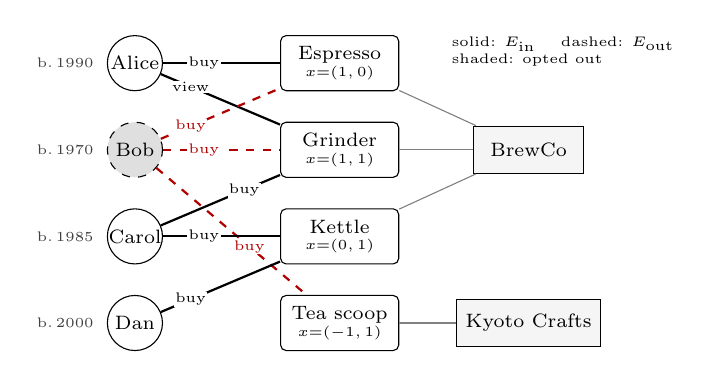
\begin{tikzpicture}[
  every node/.style={font=\scriptsize},
  cust/.style={draw, circle, minimum size=7mm, inner sep=0pt, fill=white},
  optout/.style={cust, fill=gray!25, dashed},
  item/.style={draw, rounded corners=2pt, minimum width=15mm, minimum height=7mm, fill=white, align=center, inner sep=1pt},
  merch/.style={draw, minimum width=14mm, minimum height=6mm, fill=gray!8},
  ein/.style={thick},
  eout/.style={thick, dashed, red!70!black},
  own/.style={gray, thin},
  lab/.style={font=\tiny, fill=white, inner sep=0.5pt},
  attr/.style={font=\tiny, anchor=east, text=gray!50!black}
]
\node[cust] (A) at (0,3.3) {Alice};
\node[optout] (B) at (0,2.2) {Bob};
\node[cust] (C) at (0,1.1) {Carol};
\node[cust] (D) at (0,0) {Dan};
\node[attr] at (-0.4,3.3) {b.\,1990};
\node[attr] at (-0.4,2.2) {b.\,1970};
\node[attr] at (-0.4,1.1) {b.\,1985};
\node[attr] at (-0.4,0) {b.\,2000};
\node[item] (E) at (2.6,3.3) {Espresso\\[-2pt]{\tiny $x{=}(1,0)$}};
\node[item] (G) at (2.6,2.2) {Grinder\\[-2pt]{\tiny $x{=}(1,1)$}};
\node[item] (K) at (2.6,1.1) {Kettle\\[-2pt]{\tiny $x{=}(0,1)$}};
\node[item] (S) at (2.6,0) {Tea scoop\\[-2pt]{\tiny $x{=}({-}1,1)$}};
\node[merch] (M1) at (5,2.2) {BrewCo};
\node[merch] (M2) at (5,0) {Kyoto Crafts};
\draw[ein]  (A) -- node[lab, pos=0.35]{buy} (E);
\draw[ein]  (A) -- node[lab, pos=0.25]{view} (G);
\draw[eout] (B) -- node[lab, pos=0.25]{buy} (E);
\draw[eout] (B) -- node[lab, pos=0.35]{buy} (G);
\draw[eout] (B) -- node[lab, pos=0.62]{buy} (S);
\draw[ein]  (C) -- node[lab, pos=0.7]{buy} (G);
\draw[ein]  (C) -- node[lab, pos=0.35]{buy} (K);
\draw[ein]  (D) -- node[lab, pos=0.25]{buy} (K);
\draw[own] (E) -- (M1); \draw[own] (G) -- (M1); \draw[own] (K) -- (M1);
\draw[own] (S) -- (M2);
\node[font=\tiny, align=left, anchor=west] at (3.9,3.45) {solid: $\Ein$ \quad dashed: $\Eout$\\ shaded: opted out};
\end{tikzpicture}
\caption{Running example on Monday. Customers carry an attribute (birth year) and items an intrinsic embedding $x$. Bob has opted out, so his three purchases form $\Eout$. The Tea scoop, and with it Kyoto Crafts, was bought only by Bob. Dan will opt out on Tuesday and opt back in on Friday.}
\label{fig:running}
\end{figure}

\begin{table}[t]
\centering\footnotesize
\setlength{\tabcolsep}{3pt}
\begin{tabular}{@{}llcc@{}}
\toprule
& Feature & Compliant & Bob leaks \\
\midrule
A1 & Grinder purchases & 1 & 2 \\
A1 & Kyoto Crafts sales & 0 & 1 \\
R4 & Grinder, mean birth year & 1987.5 & 1981.7 \\
\midrule
R3 & Espresso embedding & $(1,\,0.5)$ & $(0.5,\,0.5)$ \\
R3 & Grinder embedding & $(0.75,\,0.75)$ & $(0.5,\,0.83)$ \\
R3 & Kettle embedding & $(0.5,\,1)$ & $(0.5,\,1)$ \\
R3 & Tea scoop embedding & $({-}0.5,\,0.5)$ & $(0,\,0.75)$ \\
\bottomrule
\end{tabular}
\caption{Node features of Figure~\ref{fig:running}. The embedding is $F_i=\tfrac12 x_i+\tfrac12\,\mathrm{mean}\{x_j: j\text{ co-interacted with } i\}$, with the mean of an empty set taken as $0$. ``Bob leaks'' computes the same features with Bob's edges included.}
\label{tab:running}
\end{table}

\paragraph{Running example.}
Figure~\ref{fig:running} shows a toy marketplace that we reuse throughout the
paper, and Table~\ref{tab:running} computes three features on it. Alice, Carol
and Dan are opted in, and Bob is opted out. A compliant pipeline must produce
exactly the features it would produce if Bob's three dashed edges did not
exist. The Grinder's purchase count must be 1 (Carol), not 2, and its mean
customer birth year must not reflect Bob's 1970. Kyoto Crafts, whose only sale
came from Bob, must look like a merchant with no sales. The embedding is a
one-layer propagation: half the item's own $x$, half the mean $x$ of the items
that share a customer with it. Compliant, the Tea scoop has no opted-in
neighbor, so its embedding is the cold-item default $\tfrac12 x$. If Bob's
edges leak, the Tea scoop moves toward the Espresso machine and the Grinder,
and those two move toward the Tea scoop. The Kettle, which Bob never touched,
is unaffected. When Dan opts out on Tuesday, his Monday purchase of the
Kettle leaves $\Ein$ by~\eqref{eq:scope}. The Kettle's compliant purchase count
drops from 2 to 1 on Tuesday and returns to 2 on Friday.

\paragraph{Hypothesis.}
A compliant pipeline satisfies, for some measurable $f_0$,
\begin{equation}
  H_0:\; F^t = f_0(\Ein^t, x, z, \xi^t) \quad \forall t,
  \label{eq:h0}
\end{equation}
with $\xi^t$ independent of $\Eout^t$ given $\Ein^t$. Equivalently,
$F^t \indep \Eout^t \mid \Ein^t, x, z$. Every family in
Table~\ref{tab:families} reads attributes only through edges, so under $H_0$
the attributes of an opted-out customer reach no feature. The alternative is that $F^t$ depends on $\Eout^t$
through some channel. Note that this is a \emph{conditional} statement: $F$ and
$\Eout$ are marginally dependent even under $H_0$, because opted-in and
opted-out customers draw from the same preference distribution.

\paragraph{Leakage modes.}
A leak has a \emph{channel} and a \emph{pattern}. The channel is
\emph{aggregation leakage}, where counts, pooling or message passing include
some opted-out edges, or \emph{representation leakage}, where trained
parameters (embedding tables, GNN weights, factorizations) are fit on data
containing opted-out edges, even if inference later uses only $\Ein$.
Representation leakage is the harder one to detect: it need not change any
feature near an opted-out edge. Either channel leaks attributes along with
edges when the feature aggregates $z$ (R4). The pattern says which opted-out
edges leak, and it determines the \emph{leak graph}:
\begin{itemize}
  \item \emph{Per-customer leakage.} A fraction $\rho$ of opted-out customers
        leak with all of their edges, for example because one shard of the
        consent table is stale, or a status change never reached the
        pipeline. Each leaked customer contributes a whole basket, so every
        pair of her items is coupled. In Figure~\ref{fig:running}, the
        Espresso machine, the Grinder and the Tea scoop all become linked.
  \item \emph{Per-edge leakage.} Each opted-out edge leaks independently with
        probability $\rho$, for example because the consent filter runs at the
        event level and late-arriving or retried events bypass it. A pair of
        items is coupled only if \emph{both} of the customer's edges leak,
        which happens with probability $\rho^2$. If only Bob's Grinder
        purchase leaks, the Grinder's count rises, but no pair of items is
        linked through Bob.
\end{itemize}
The two patterns produce the same aggregation leaks per edge, but very
different leak graphs, and therefore different power for tests that look at
pairs (Section~\ref{sec:did}).

\paragraph{What cannot be shown.}
Could an auditor ever \emph{certify} that a pipeline is compliant? The answer
is no, and the reason shapes everything that follows.

Testing $H_0$ is a conditional-independence (CI) test: we ask whether $F$
still depends on $\Eout$ once $\Ein$ is known. \citet{shah2020hardness} prove
that CI testing is hard in a strong sense. When the conditioning variable is
continuous, any test that keeps its false-positive rate at most $\alpha$ under
\emph{every} null distribution has power at most $\alpha$ against \emph{every}
alternative. Put simply, a test cannot be both always valid and ever useful
unless we add assumptions about what the data can look like. Their result
concerns general distributions, and our setting has extra structure (a graph
and a fixed pipeline), so we do not rely on it directly. A more elementary
argument fits our setting and gives a concrete number.

Picture a buggy pipeline $f_1$ that behaves exactly like a compliant $f_0$
except on rare inputs. In Figure~\ref{fig:running}, $f_1$ might include
Bob's purchases only when a nightly job retries after a timeout and skips the
consent join. On every other day the two pipelines produce identical outputs,
so no statistic of the outputs can tell them apart on those days.

\begin{proposition}[No certificate of zero use]\label{prop:imposs}
Let $f_0$ satisfy $H_0$, and let $f_1$ agree with $f_0$ except on an input event of
per-day probability at most $\delta$, on which it uses $\Eout$ arbitrarily. For any
test $\phi$ of level $\alpha$ against $f_0$ on $T$ days,
$\Pr_{f_1}[\phi=1]\le \alpha+T\delta$.
\end{proposition}
\begin{proof}[Proof sketch]
Couple the two pipelines on the same inputs and randomness. Their outputs
differ only on the union of the per-day events, which has probability at most
$T\delta$. Hence the total-variation distance between the laws of
$\mathcal{D}_T$ is at most $T\delta$, and the acceptance probabilities differ by at most
that much.
\end{proof}
For a concrete sense of scale, suppose the retry bug fires on one day in a
thousand ($\delta=0.001$) and the audit runs for a 30-day quarter. Then
\emph{every} level-0.05 test detects it with probability at most
$0.05+0.03=0.08$, however clever the test. More generally, the auditor cannot
distinguish ``never leaks'' from ``leaks rarely enough.'' The same argument
covers a deliberately evasive pipeline, which can make its leaking event as
rare as it likes. Black-box auditing is therefore a tool against \emph{bugs},
not adversarial pipelines. Bugs tend to be systematic: a missing filter
affects every day and many nodes, which is what makes them detectable. The
honest output of an audit is a statement of the form ``leakage of magnitude
at least $\varepsilon$ would have been detected with probability at least
$1-\beta$; none was.''

%=====================================================================
\section{Naive Tests and Their Pitfalls}\label{sec:challenges}
%=====================================================================
An auditor's first tests follow two simple ideas. The first looks at a single
node: if only its opted-out edges changed, its feature should not change
(Section~\ref{sec:single}). The second compares groups: items that opted-out
customers connect should look no different from a reference group
(Section~\ref{sec:did}). Both ideas are sound, and Section~\ref{sec:tests}
builds on both. Their naive versions, however, fall into five pitfalls, each a
heuristic that sounds right but is false for real pipelines. For each, we give
a positive example where the naive test catches a real leak in
Figure~\ref{fig:running}, a counterexample where it raises a false alarm on a
compliant pipeline, and the false-alarm rate we measure on compliant
pipelines, in our simulator and on real data (Section~\ref{sec:naive}).
Table~\ref{tab:challenges} summarizes them. We focus on representations:
aggregations are the easy case, and the single-node test is exact for them.

\begin{table}[t]
\centering\footnotesize
\setlength{\tabcolsep}{3pt}
\begin{tabular}{@{}l>{\raggedright}p{1.55in}>{\raggedright\arraybackslash}p{0.95in}@{}}
\toprule
& Heuristic (false in general) & Fix \\
\midrule
\multicolumn{3}{@{}l}{\emph{Single node} (Section~\ref{sec:single})}\\
P1 & unchanged opted-in edges $\Rightarrow$ unchanged feature & $k$-hop invariance, control group \\
P2 & unchanged embedding $\Rightarrow$ unchanged coordinates & alignment \\
P3 & same input $\Rightarrow$ same output & fixed seed, control group \\
\midrule
\multicolumn{3}{@{}l}{\emph{Difference in differences} (Section~\ref{sec:did})}\\
P4 & opted-out pairs are no closer than random pairs & placebo with the same structure \\
P5 & tomorrow's interactions are a fair, independent reference & customer units, bracketing \\
\bottomrule
\end{tabular}
\caption{Five heuristics behind naive tests, and the fixes used in Section~\ref{sec:tests}. Table~\ref{tab:naive} measures each failure.}
\label{tab:challenges}
\end{table}

\subsection{Single-node tests}\label{sec:single}
\paragraph{The idea.}
Under $H_0$, a node's feature is a function of opted-in data only. If nothing
opted in changed around a node and only its opted-out edges changed, a
compliant pipeline has no reason to change its feature. A change is then
evidence that the pipeline read the opted-out edges.

\paragraph{The naive test.}
Each night, find items whose typed opted-in edges are identical on days $t$
and $t{+}1$ but whose opted-out edges changed. Flag a leak if any of these
items' embeddings changed. Restricting to items with no opted-in change is
essential: without it, legitimate changes would trigger the test every day.

\paragraph{When it works.}
Take the embedding of Table~\ref{tab:running}, computed deterministically.
On Tuesday, Bob buys the Kettle. Carol's and Dan's edges with the Kettle are
unchanged, so the Kettle qualifies. A compliant pipeline ignores Bob's new
edge, and the Kettle stays at $(0.5,\,1)$. A leaking pipeline adds Bob's other
items to the Kettle's neighbors and moves it toward the Espresso machine, the
Grinder and the Tea scoop. The test sees the change and correctly flags the
leak. For aggregations (A1, A2), the test is exact and always valid: a count
over an item's own opted-in edges cannot change if those edges did not.

\paragraph{Pitfall 1: ``Unchanged opted-in edges mean an unchanged feature.''}
This holds only for features that read nothing beyond the node's own edges.
An embedding also reads its neighbors' edges. On Tuesday, Carol also buys a
teapot. The Kettle's own opted-in edges are unchanged, but Carol now connects
it to the teapot, so its propagated embedding legitimately moves. Since Bob
touched the Kettle the same day, the test blames him. For a $k$-layer GNN,
everything within $k$ hops matters; for a factorization fit on the whole
graph (R1, R2), every edge does. In our simulator, the deterministic
one-layer propagation alarms on 28\% of compliant days with the naive 1-hop
check, and on 0\% when invariance is checked over 2 hops; on real data, where
neighbors' baskets change constantly, on 100\% and 0\% (Table~\ref{tab:naive}).

\paragraph{Pitfall 2: ``An unchanged embedding means unchanged coordinates.''}
Embeddings that are retrained each day have no fixed coordinates. Suppose
Tuesday's factorization produces exactly Monday's geometry, but rotated. All
distances and angles are unchanged, yet every coordinate of every item
differs, and the test flags the entire catalog. Aligning the two days'
spaces, e.g., with orthogonal Procrustes~\citep{schonemann1966procrustes}, or
comparing only rotation-invariant quantities, such as norms and cosine
similarities, removes this. On randomly retrained factorizations, alignment
cuts the median relative change of input-unchanged items from 1.40 to 0.014.

\paragraph{Pitfall 3: ``The same input gives the same output.''}
Many pipelines are random: they initialize from a fresh seed, sample
negatives or mini-batches, or run a randomized SVD. Even run twice on the same
input, they give every item a slightly different embedding, and the test
fires on noise. This pitfall has an easy fix when the operator controls the
pipeline: fix the random seed in the audited run. Fixing the seed is not
enough on its own, however. A factorization (R1) with a fixed seed still
alarms on 100\% of simulated and real days, before and after alignment, because the
global fit moves with every opted-in change anywhere in the graph
(Pitfall~1 again).

\paragraph{Ideas for the fix.}
Pitfalls 1--3 share one remedy. Instead of asking whether a feature changed,
ask whether it changed \emph{more} than the features of comparable nodes whose
opted-out edges did not change. Select items whose opted-in input is
unchanged over the pipeline's receptive field ($k$ hops), align the two days,
and compare these treated items with control items. Global retraining, noise
and rotation then move both groups alike. In Section~\ref{sec:tests} we turn
this into T2. On randomly retrained factorizations it alarms on 6\% of
simulated and 7\% of real days at $\alpha=0.05$, against 100\% for the naive
test.

\subsection{Difference in differences}\label{sec:did}
\paragraph{The idea.}
A representation leak need not change any single node visibly, but it changes
\emph{relations}: training on an opted-out customer's basket pulls her items
together. So compare the items that opted-out customers connect with a
reference group. The difference between the two groups, relative to the
difference expected without a leak, measures the leak.

\paragraph{The naive test.}
Take every pair of items co-purchased by an opted-out customer, and check
whether these pairs are closer in feature space than random item pairs.

\paragraph{When it works.}
Suppose the pipeline trains on all edges, including Bob's. Bob is the only
link between the Grinder and the Tea scoop. In Table~\ref{tab:running}, the
leak moves the Tea scoop from $({-}0.5,\,0.5)$ to $(0,\,0.75)$, and its cosine
similarity with the Grinder rises from 0 to 0.86. The test finds the pair
unusually close and correctly flags the leak.

\paragraph{Pitfall 4: ``Pairs co-purchased by opted-out customers should be no closer than random pairs.''}
This fails because opted-in and opted-out behavior are correlated. Alice
bought the Espresso machine and viewed the Grinder, so a compliant pipeline
places the two close together using her edges alone. Bob also bought both, so
the pair counts as an opted-out co-purchase, and the test fires anyway. On
compliant pipelines, the naive test alarms on 100\% of days, in our simulator
and on real data (Table~\ref{tab:naive}). A stricter version keeps only pairs
that \emph{only} opted-out customers co-purchased, so that no opted-in
customer bought both items. This removes the Espresso machine--Grinder pair.
It still alarms on 94\% of simulated and 100\% of real days, for four reasons.
\begin{itemize}
  \item \emph{Indirect opted-in paths.} The Grinder and the Tea scoop were
        never bought together by an opted-in customer. But if Dan also bought
        the Tea scoop, the two would be linked through Carol and Dan:
        Grinder--Carol--Kettle--Dan--Tea scoop. Matrix
        factorization~\citep{koren2009matrix}, skip-gram
        embeddings~\citep{barkan2016item2vec,levy2014neural}, GNNs and feature
        propagation~\citep{hamilton2017graphsage,he2020lightgcn} all encode
        such transitive similarity. In our simulator, 99\% of the pairs that
        pass the stricter filter are still linked by a short opted-in path, and
        these pairs carry all of the residual gap.
  \item \emph{Shared taste and content.} Bob's basket reflects his
        preferences, so its items are related in their intrinsic embeddings
        $x$. A pipeline that feeds $x$ into $F$ makes them similar even with no
        opted-in path at all.
  \item \emph{Selection.} A popular item is bought by many opted-in
        customers, so for almost any pair that contains it, some opted-in
        customer bought both items. The filter therefore removes nearly every
        pair that involves a popular item. The surviving pairs consist of
        niche items, which differ from random pairs in degree and in how noisy
        their embeddings are.
  \item \emph{Coverage.} The test only sees leaks that couple two items. It is
        blind to aggregation leaks, such as an inflated purchase count, which
        change no pairwise similarity. Its power also depends on the leak
        pattern: under per-customer leakage each leaked customer couples all
        of her pairs, so the signal grows with $\rho$; under per-edge leakage a
        pair is coupled only if both of its edges leak, so the signal grows
        with $\rho^2$.
\end{itemize}

\paragraph{Pitfall 5: ``Tomorrow's interactions are a fair, independent reference.''}
A better reference than random pairs has the same structure but no possible
leak: for instance, pairs that customers co-purchase only \emph{tomorrow},
which today's pipeline cannot have seen. In our simulator, where customers
draw baskets independently from stationary preferences, such tests are close
to calibrated, with false alarms on 2--4\% of days. Real behavior breaks the
heuristic in three ways. First, units are dependent: browsing comes in
sessions, and one customer contributes many correlated pairs and edges, so
treating them as independent overstates the evidence. Second, behavior
drifts: this week's items differ from next week's, so tomorrow's interactions
are not exchangeable with today's. On RetailRocket, the same tests alarm on
29\% (pairs) and 13\% (edges) of compliant days. Third, the reference can be
selected. Edges defined as ``present tomorrow but not today'' exclude, by
construction, the items a customer keeps buying, which are the items most
similar to the rest of her basket. In the simulator, this alone makes a
customer's suspect edges look closer to her basket than her reference edges,
and a test against a compliant co-occurrence embedding (R2) alarms on 17 of
20 days.

\paragraph{Ideas for the fix.}
A stricter filter on the suspect pairs cannot remove the confounding of
Pitfall~4. What works is a reference group with the same tastes, the same
indirect paths and the same sparsity, but no possible leak. Pitfall~5 then
dictates how to build and use it: take the customer as the unit; bracket the
window in time, drawing references both from interactions that just
\emph{left} the window and from those that \emph{enter} it next; and select
suspect and reference units by the same rule. In Section~\ref{sec:tests} we
introduce two tests built this way: a co-occurrence test with a temporal
placebo (T5) and an edge-level membership test (T6). With these refinements,
neither raises a false alarm on real data (Section~\ref{sec:real}).

%=====================================================================
\section{Audit Tests}\label{sec:tests}
%=====================================================================
We make one structural assumption, stated for item features; customer and
merchant features are analogous.

\begin{assumption}[Locality given global state]\label{ass:local}
There exist a radius $k\ge 1$ and two fixed functions $\theta$ and $\varphi$,
both unknown to the auditor, such that under $H_0$, for every node $v$ and day
$t$,
\begin{equation}
  F_v^t=\varphi\big(\N_k^{\mathrm{in}}(v),\, x_v,\, \Theta^t,\, \xi_v^t\big),
  \qquad \Theta^t=\theta(\Ein^t,\xi^t).
  \label{eq:local}
\end{equation}
Here $\N_k^{\mathrm{in}}(v)$ is the typed $k$-hop neighborhood of $v$ in $\Ein^t$,
$\Theta^t$ is a global state such as trained parameters, and $\xi_v^t$ is the
part of the pipeline's randomness $\xi^t$ that acts on node $v$.
\end{assumption}

Assumption~\ref{ass:local} refines the compliant pipeline $f_0$ in
\eqref{eq:h0} by splitting it into two stages. The \emph{training} stage
$\theta$ may look at all of $\Ein^t$ and produces global state $\Theta^t$. The
\emph{readout} stage $\varphi$ computes each node's feature from that state and
the node's own $k$-hop opted-in neighborhood. For a two-layer GraphSAGE model,
for example, $\theta$ is the training run, $\Theta^t$ are the learned weights,
$\varphi$ is the forward pass, and $k=2$. For a purchase count, $\Theta^t$ is
empty, $\varphi$ counts typed edges, and $k=1$. Since the pipeline is fixed,
$\theta$ and $\varphi$ are the same functions every day and for every node. The
tests rely on exactly this: in Figure~\ref{fig:running}, the Tea scoop's
feature is $\varphi(\emptyset, x_{\text{scoop}}, \Theta^t, \xi^t_{\text{scoop}})$,
the same function applied to a never-bought item. The assumption rules out no
leakage mode. It only says where, under $H_0$, information may come from.
Table~\ref{tab:tests} summarizes the tests. Each test ends with a short
paragraph, \emph{Avoiding the pitfalls}, that explains how its design escapes
the naive-test failures of Section~\ref{sec:challenges}.

\begin{table}[t]
\centering\small
\setlength{\tabcolsep}{3pt}
\begin{tabular}{@{}llll@{}}
\toprule
Test & Targets & Needs & Key control \\
\midrule
T1 canary & agg., repr. & long tail & empty $\N^{\mathrm{in}}$ \\
T2 zero-diff & agg., repr. & churn & invariant $\N_k^{\mathrm{in}}$ \\
T3 DiD & agg. & status switches & matched items \\
T4 residual & agg. & --- & surrogate of $\Ein$ \\
T5 co-occur. & repr. & --- & temporal placebo \\
T6 edge MI & repr. & basket churn & same-user fresh edges \\
T7 active (ref.) & any & write access & random assignment \\
\bottomrule
\end{tabular}
\caption{Audit tests, the leakage modes they target, what they require, and the control that makes them valid under $H_0$. T1--T6 are passive; T7 is the active reference.}
\label{tab:tests}
\end{table}

\subsection{T1: Natural canaries}
T1 uses nodes whose correct output is known in advance.

\paragraph{Natural canary.}
An item is a \emph{natural canary} on day $t$ if it has at least one opted-out
edge and no opted-in edge. In Figure~\ref{fig:running}, the Tea scoop is a
canary, because only Bob bought it. The same idea applies at other levels.
Kyoto Crafts is a merchant-level canary, because all of its sales came from
opted-out customers. Every opted-out customer, such as Bob, is a
customer-level canary.

\paragraph{Cold item.}
A \emph{cold} item is one that nobody touched on day $t$, such as a newly listed
item.

\paragraph{The test.}
Under $H_0$, the pipeline receives exactly the same input for a canary as for a
cold item: an empty receptive field. By Assumption~\ref{ass:local}, both get
the feature $\varphi(\emptyset, x_i, \Theta^t, \xi_i^t)$, from the same function. So
canaries and cold items with similar intrinsic features must be
indistinguishable. In Figure~\ref{fig:running}, the Tea scoop's purchase count
must be 0, and its embedding must look like that of a never-bought tea
accessory. Kyoto Crafts must look like a merchant with no sales, and Bob's
customer feature must equal the default given to a customer with no history.
If the Tea scoop's count is 1, or its embedding sits next to the Grinder
(Bob's other purchase), then Bob's edges leaked.

\paragraph{Implementation.}
We compare canaries with cold items using a permutation test on the feature
norm, matching or adjusting on $x_i$. For customers, the default output is
deterministic in our pipelines, so an exact check applies: any opted-out
customer whose feature differs from the default is a violation. Long-tailed
catalogs supply dozens of new canaries every day: 34 per day in our
simulation.

\paragraph{Avoiding the pitfalls.}
T1 is the most robust passive test, because canaries and cold items receive
the same, empty, opted-in input. Correlated behavior (P4) therefore cannot make
them differ, and neither can changes elsewhere in the graph (P1), which reach
both groups only through the same global state. One residual form of P4
remains: someone \emph{chose} to buy the Tea scoop, so canaries may be
intrinsically more attractive than cold items. This is why we match on $x_i$.
Finally, the feature norm is unchanged by rotations of the embedding space
(P2), so no alignment is needed.

\subsection{T2: Zero-difference on invariant neighborhoods}
T2 compares how much features move overnight for two groups of items whose
opted-in inputs did not change. It needs two definitions.

\paragraph{Receptive field.}
Under Assumption~\ref{ass:local}, the only opted-in data that can affect
$F_v^t$ \emph{locally} is $\N_k^{\mathrm{in}}(v)$: the typed opted-in edges within $k$
hops of $v$. Everything else reaches $v$ only through the global state
$\Theta^t$. We call $\N_k^{\mathrm{in}}(v)$ the \emph{receptive field} of $v$. In
Figure~\ref{fig:running}, suppose the pipeline is a two-layer GNN ($k=2$).
The Grinder's receptive field then contains its own opted-in edges (Alice's
view, Carol's purchase) and the other opted-in edges of those customers
(Alice's purchase of the Espresso machine, Carol's purchase of the Kettle).
Dan's purchase of the Kettle is three hops away and lies outside it. For a
purchase count ($k=1$), the receptive field is just the item's own opted-in
edges.

\paragraph{Opted-out neighborhood.}
Let $\N^{\mathrm{out}}(v)$ be the set of typed opted-out edges incident to $v$. The
Espresso machine's opted-out neighborhood is $\{(\text{Bob}, \text{buy})\}$. It
\emph{changes} between two days when an opted-out customer adds, removes or
changes the type of an interaction with the item. If Bob also reviews the
Espresso machine on Tuesday, its opted-out neighborhood becomes
$\{(\text{Bob},\text{buy}), (\text{Bob},\text{review})\}$.

\paragraph{The test.}
Select items whose receptive field is identical on days $t$ and $t{+}1$. Under
$H_0$, the features of these items can still move, but only because $\Theta$ was
retrained and because of noise. Those causes affect all selected items
alike. Split the selected items into two groups. \emph{Treated} items have a
changed opted-out neighborhood, and \emph{control} items do not. A compliant
pipeline never reads the opted-out edges, so treated items should move no
more than control items. In Figure~\ref{fig:running}, if Bob reviews the
Espresso machine on Tuesday and nothing in its receptive field changes, the
Espresso machine is treated. If its embedding moves noticeably more than those
of comparable control items, Bob's review leaked.

To implement the test, we align the two days' embeddings, compute each
item's relative change $\|\Delta F_i\|/\|F_i\|$, and regress its logarithm on
the treatment indicator and log degree. We then test whether the treatment
coefficient is positive. For a deterministic 1-hop aggregate, no regression
is needed: any change in a treated item's count is a violation, which gives an
exact test. Treatment is defined by the item's \emph{own} opted-out edges,
because those are the ones a leak affects most. Opted-out changes farther away
may also move control items under a leak. That dilutes the contrast and costs
power, but it cannot cause false alarms.

\paragraph{Avoiding the pitfalls.}
The control group measures the noise floor, so random retraining (P3) moves
both groups alike. Embeddings are aligned before comparison (P2). Invariance is
checked over the full receptive field, not just direct neighbors (P1), and on
typed edges, since a pair can change type (Section~\ref{sec:problem}). Finally, treated and control items have identical opted-in
inputs on both days, so correlated behavior (P4) cannot separate them.

\subsection{T3: Status-switch difference-in-differences}
T3 checks that a customer's contribution disappears, or appears, on the day
their status changes.

\paragraph{Status switch.}
A customer \emph{switches} when their opt-out status changes between days $t$ and
$t{+}1$. In Figure~\ref{fig:running}, Dan opts out on Tuesday. Under a
retroactive scope of Section~\ref{sec:problem}, all of Dan's edges move from
$\Ein$ to $\Eout$ on that day. Call the items Dan touched \emph{affected} items.
Here, the Kettle is affected.

\paragraph{The reference change, without a formula.}
The auditor cannot compute how the Kettle's feature \emph{should} change,
because it does not know the pipeline. A compliant pipeline, however, sees
Dan's switch exactly as if Dan had deleted his interactions: one opted-in
purchase disappears from the Kettle. Items lose opted-in edges for ordinary
reasons every day, for instance when a customer's basket changes. These
\emph{natural removals} show, empirically, how the pipeline responds to losing
an edge of a given type. For each affected item, we therefore select
\emph{comparison} items that lost the same number and types of opted-in edges
that day for ordinary reasons, matched on degree. Suppose the Toaster lost one
purchase on Tuesday because its buyer's basket changed. A compliant pipeline
must treat the Kettle and the Toaster alike: whatever happens to the Toaster's
purchase count and embedding on Tuesday should also happen to the Kettle's.
Switches back to opt-in work the same way, with \emph{natural additions} as the
reference: when Bob opts back in, his items should respond like items that
gained the same opted-in edges for ordinary reasons. With many days of data,
the auditor can go further and fit a model of the pipeline's response,
$\Delta F_i$ as a function of the change in item $i$'s typed opted-in edge counts,
on items that no switch affected, and use it to predict the affected items'
change.

\paragraph{The test.}
We compare affected and comparison items in a difference-in-differences
design~\citep{angrist2009mostly}, using the change from $t$ to $t{+}1$ and on the
following days. Compliance predicts that affected items respond on the switch
day exactly as comparison items do, and that neither group shows further
change afterwards. Two bugs produce different patterns:
\begin{itemize}
  \item \emph{Stale cache or delayed deletion.} On Tuesday, the Toaster's count
        drops but the Kettle's does not, because the pipeline still uses Dan's
        purchase. The Kettle catches up only on Thursday. Affected items
        respond \emph{less} than comparison items on the switch day, and
        \emph{more} on later days.
  \item \emph{Opted-out data used before an opt-in.} Bob opts back in on
        Thursday, so his edges legitimately join $\Ein$ on Thursday. If his items
        already carried his signal on Wednesday, they respond \emph{less} than
        comparison items on Thursday, because there is nothing left to add.
\end{itemize}
For deterministic columns, such as counts, the comparison items also reveal
how the column responds to one removed edge. If every comparison item's count
drops by one, a single affected item whose count does not drop is a
violation.

\paragraph{Avoiding the pitfalls.}
Comparison items have the same kind of opted-in change on the same day, so
correlated behavior (P4) and retraining noise (P3) affect both groups alike.
Embeddings are aligned before comparison (P2). Edge changes are matched on type,
and the opt-out scope is fixed in advance (Section~\ref{sec:problem}).

\paragraph{What it adds.}
T3 targets how status changes propagate through the pipeline: stale consent
tables, caches and delayed deletions. Such bugs can pass T1 and T2 on days
without switches. Our simulated pipelines have no caching, so we do not
evaluate T3 in Section~\ref{sec:exp}.

\subsection{T4: Residual regression with surrogate controls}
T4 asks whether $F$ knows something about opted-out edges that $\Ein$ cannot
explain.

\paragraph{Opted-out summary.}
For each item, let $S^{\mathrm{out}}_i=\log(1+|\N^{\mathrm{out}}(i)|)$ summarize its opted-out
edges. In Figure~\ref{fig:running}, $|\N^{\mathrm{out}}(i)|$ is 1 for the Espresso machine,
the Grinder and the Tea scoop, and 0 for the Kettle.

\paragraph{Surrogate features.}
The auditor computes its own features $Z_i$ from $\Ein$ and $x$ alone: typed
counts, its own factorization of $\Ein$, and a propagation of $x$ over $\Ein$. For
the Grinder, $Z$ encodes that Alice viewed it, that Carol bought it, and that
it resembles the Espresso machine.

\paragraph{The test.}
Fit two predictors of $S^{\mathrm{out}}$. Model A uses $Z$ only, and model B uses $Z$ and
$F$. Under $H_0$, $F$ is a function of $\Ein$ plus noise. If $Z$ captures what $\Ein$
says about $S^{\mathrm{out}}$, model B cannot beat model A on held-out items. If it does,
$F$ carries opted-out information. For example, suppose the pipeline reports a
purchase count of 2 for the Grinder, while the auditor's count from $\Ein$ is 1.
Model B then learns that the difference between the two counts predicts
$S^{\mathrm{out}}$ exactly.

\paragraph{Implementation.}
We use ridge regression with 5-fold cross-fitting, in the spirit of double
machine learning~\citep{chernozhukov2018double}. We compute the per-item
difference in held-out squared error between the two models and apply a
one-sided $t$-test. It suits aggregates best. Against representation leakage
it is weak, because a count of opted-out edges discards \emph{which} edges
leaked.

\paragraph{Avoiding the pitfalls.}
The surrogate $Z$ is what protects T4 against correlated behavior (P4). Model A
already uses everything $Z$ knows about $\Ein$, so model B can only win with
information that $Z$ lacks. The protection is only as good as $Z$. If $F$
encodes opted-in information that $Z$ misses, false alarms are possible. In our
experiments the test is conservative. Both models predict a per-item target
from a single day's features, so randomness (P3) and rotations (P2) act as
noise, not bias.

\begin{figure*}[t]
\centering
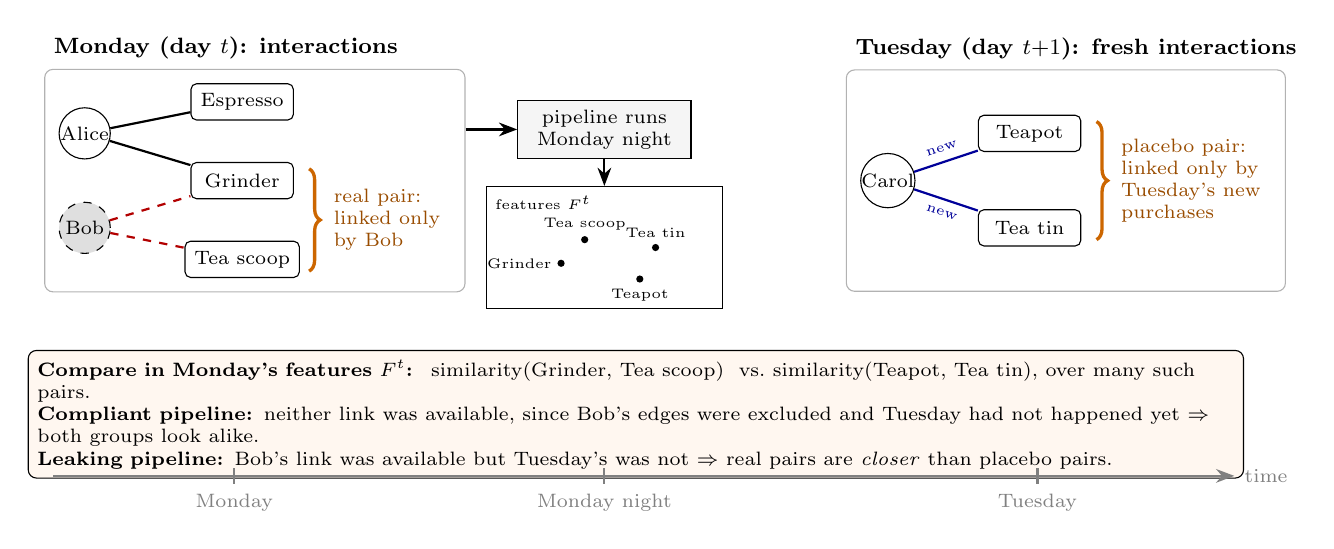
\begin{tikzpicture}[
  every node/.style={font=\scriptsize},
  cust/.style={draw, circle, minimum size=6.5mm, inner sep=0pt, fill=white},
  optout/.style={cust, fill=gray!25, dashed},
  item/.style={draw, rounded corners=2pt, minimum width=13mm, minimum height=4.6mm, fill=white},
  ein/.style={thick},
  eout/.style={thick, dashed, red!70!black},
  fresh/.style={thick, blue!60!black},
  panel/.style={draw, gray!60, rounded corners=3pt, inner sep=5pt},
  ttl/.style={font=\footnotesize\bfseries, anchor=south west}
]
% ---- Panel A: Monday interactions
\node[cust]   (A)  at (0,1.6) {Alice};
\node[optout] (B)  at (0,0.4) {Bob};
\node[item]   (E)  at (2.0,2.0) {Espresso};
\node[item]   (G)  at (2.0,1.0) {Grinder};
\node[item]   (S)  at (2.0,0.0) {Tea scoop};
\draw[ein]  (A) -- (E); \draw[ein] (A) -- (G);
\draw[eout] (B) -- (G); \draw[eout] (B) -- (S);
\draw[orange!80!black, very thick, decorate, decoration={brace, amplitude=4pt}] (2.85,1.15) -- (2.85,-0.15)
  node[midway, right=5pt, align=left, text=orange!60!black] (RL) {real pair:\\linked only\\by Bob};
\begin{scope}[on background layer]
\node[panel, fit=(A)(B)(E)(S)(G)(RL)] (PA) {};
\end{scope}
\node[ttl] at (PA.north west) {Monday (day $t$): interactions};

% ---- Panel B: pipeline + features
\node[draw, fill=gray!8, minimum width=2.2cm, minimum height=7mm, align=center] (P) at (6.6,1.65) {pipeline runs\\Monday night};
\node[draw, minimum width=3.0cm, minimum height=1.55cm] (FB) at (6.6,0.15) {};
\node[font=\tiny, anchor=north west] at (FB.north west) {features $F^{t}$};
\fill (6.05,-0.05) circle (1.3pt) node[left, font=\tiny] {Grinder};
\fill (6.35,0.25) circle (1.3pt) node[above, font=\tiny] {Tea scoop};
\fill (7.05,-0.25) circle (1.3pt) node[below, font=\tiny] {Teapot};
\fill (7.25,0.15) circle (1.3pt) node[above, font=\tiny] {Tea tin};
\draw[-{Stealth}, thick] (P) -- (FB);
\draw[-{Stealth}, thick] (PA.east |- P) -- (P.west);

% ---- Panel C: Tuesday fresh interactions
\node[cust] (C)  at (10.2,1.0) {Carol};
\node[item] (TP) at (12.0,1.6) {Teapot};
\node[item] (TT) at (12.0,0.4) {Tea tin};
\coordinate (Ctop) at (10.2,2.23); \coordinate (Cbot) at (10.2,-0.23);
\draw[fresh] (C) -- node[above, sloped, font=\tiny]{new} (TP);
\draw[fresh] (C) -- node[below, sloped, font=\tiny]{new} (TT);
\draw[orange!80!black, very thick, decorate, decoration={brace, amplitude=4pt}] (12.85,1.75) -- (12.85,0.25)
  node[midway, right=5pt, align=left, text=orange!60!black] (PL) {placebo pair:\\linked only by\\Tuesday's new\\purchases};
\begin{scope}[on background layer]
\node[panel, fit=(C)(TP)(TT)(PL)(Ctop)(Cbot)] (PC) {};
\end{scope}
\node[ttl] at (PC.north west) {Tuesday (day $t{+}1$): fresh interactions};

% ---- comparison
\node[draw, rounded corners=3pt, fill=orange!6, align=left, text width=15.2cm, anchor=north] (CMP) at (7.0,-1.15)
{\textbf{Compare in Monday's features $F^{t}$:} \ similarity(Grinder, Tea scoop) \ vs.\ similarity(Teapot, Tea tin), over many such pairs.\\
\textbf{Compliant pipeline:} neither link was available, since Bob's edges were excluded and Tuesday had not happened yet $\Rightarrow$ both groups look alike.\\
\textbf{Leaking pipeline:} Bob's link was available but Tuesday's was not $\Rightarrow$ real pairs are \emph{closer} than placebo pairs.};

% ---- time axis
\draw[-{Stealth}, thick, gray] (-0.4,-2.75) -- (14.6,-2.75) node[right, text=gray] {time};
\foreach \x/\l in {1.9/Monday, 6.6/Monday night, 12.1/Tuesday}
  \draw[gray, thick] (\x,-2.65) -- (\x,-2.85) node[below, text=gray] {\l};
\end{tikzpicture}
\caption{The temporal placebo of T5. Real pairs are linked only through opted-out customers on day $t$. Placebo pairs are linked only through interactions that first appear on day $t{+}1$, after day $t$'s features were computed. Both kinds of pair arise from the same shopping behavior, so they share any taste-driven similarity. Only the real pairs could have leaked.}
\label{fig:t5}
\end{figure*}

\subsection{T5: Co-occurrence membership inference with a temporal placebo}
T5 targets representation leakage. Training on Bob's basket pulls together
the items Bob bought together, much as membership-inference attacks detect
training data~\citep{shokri2017membership,carlini2022first}. On graphs, the
natural unit is a co-interaction~\citep{he2021stealing,olatunji2021membership}.

\paragraph{Real pairs.}
Let $\mathcal{R}^t$ contain the item pairs that are co-purchased \emph{only} through
opted-out customers on day $t$, and never together in $\Ein^t$. In
Figure~\ref{fig:running}, (Grinder, Tea scoop) is a real pair, because only Bob
bought both.

\paragraph{Placebo pairs.}
Comparing real pairs with random item pairs is the naive test of Pitfall~4, and it
fails because shared taste makes real pairs similar anyway. We therefore
need a reference group with the same taste-driven similarity but no possible
leak. Let $\mathcal{Q}^t$ contain the pairs that co-occur only through interactions
that first appear on day $t{+}1$, which the day-$t$ pipeline could not have seen.
For example, if Carol buys a teapot and a tea tin together on Tuesday, then
(teapot, tea tin) is a placebo pair for Monday. Placebo pairs come from the
same behavior that produces real pairs, so they share the taste-driven
similarity that broke the naive test, but they cannot have leaked into
Monday's features. Figure~\ref{fig:t5} shows the timeline.

\paragraph{The test.}
Compare the cosine similarity of real and placebo pairs in $F^t$. Under $H_0$ the
two distributions are the same. If real pairs are systematically closer, the
pipeline learned from opted-out baskets.

\paragraph{Implementation.}
Two details are essential. First, the two groups must use symmetric
exclusions. Neither may co-occur in $\Ein^t$. Real pairs exclude pairs that also
co-occur in day $t{+}1$'s fresh interactions, and placebo pairs exclude pairs
that also co-occur in $\Eout^t$. Second, overlapping pairs share items and are
therefore dependent, which makes standard errors too small. We subsample pairs
so that no item appears twice. We then regress similarity on group membership
and the two items' log degrees, and test the group coefficient.
Section~\ref{sec:exp} shows that both details are necessary. Real data needs
two further refinements (P5). First, each customer contributes at most one
pair, because pairs from one browsing session are correlated. Second, the
placebo brackets the window in time. It combines pairs that co-occur only
through interactions that \emph{left} the window on day $t$ with pairs that
co-occur only through interactions that \emph{enter} it on day $t{+}1$.

\paragraph{Avoiding the pitfalls.}
The placebo absorbs correlated behavior (P4). Both groups are scored with
the same day's features, so randomness (P3) affects them alike. Cosine
similarity within one embedding space is unchanged by rotations (P2).

\subsection{T6: Edge-level membership inference}
T6 asks directly whether the pipeline \emph{remembers} individual opted-out edges.
It applies the logic of membership inference: a trained model tends to score
its training data higher than data it never
saw~\citep{shokri2017membership,carlini2022first}.

\paragraph{Scoring an edge.}
For an edge $(u,i)$ on day $t$, the auditor builds a context vector for customer
$u$ from $F$ alone: the mean embedding of $u$'s other items that day. The edge's
score is the cosine similarity between item $i$'s embedding and this context.
In Figure~\ref{fig:running}, Bob's edge to the Tea scoop is scored by
comparing the Tea scoop's embedding with the mean embedding of the Espresso
machine and the Grinder. The context is needed because a compliant pipeline
gives Bob only the default customer feature (T1).

\paragraph{Three groups of edges.}
\begin{itemize}
  \item \emph{Members} (IN): opted-in edges on day $t$. The pipeline legitimately
        learns from them, so they score high if it memorizes edges.
  \item \emph{Suspects} (OUT): opted-out edges on day $t$, such as Bob's three
        purchases.
  \item \emph{Guaranteed non-members} (FRESH): for opted-out customers whose
        basket changes on day $t{+}1$, their day-$(t{+}1)$ basket, scored with
        day-$t$ features. The day-$t$ pipeline cannot have seen these
        interactions.
\end{itemize}

\paragraph{The test.}
We compare OUT with FRESH, not with IN. Under $H_0$, both are non-members.
They come from the same customers with the same tastes, so they score alike.
Under a leak, OUT edges become members and score higher. For each opted-out
customer with both kinds of edge, we compute the difference between the mean
OUT score and the mean FRESH score. We then test whether these differences are
positive across customers (one-sided $t$-test). Comparing OUT with IN directly
would not work. How much higher members score than non-members depends on how
much the pipeline memorizes. A pipeline that generalizes smoothly scores
members and non-members alike even when it is compliant, so ``OUT looks like
IN'' would not imply a leak. FRESH supplies the missing reference.

\paragraph{An effect size.}
IN provides a scale. Let INF be the next-day baskets of opted-in customers,
scored the same way, and let $\bar s$ denote a group's mean score. Define
\begin{equation}
  \lambda=\frac{\bar s_{\mathrm{OUT}}-\bar s_{\mathrm{FRESH}}}{\bar s_{\mathrm{IN}}-\bar s_{\mathrm{INF}}}.
\end{equation}
$\lambda\approx 0$ under compliance, and $\lambda\approx 1$ when the pipeline treats all
opted-out edges as training data. In between, $\lambda$ roughly estimates the
fraction of opted-out edges that behave like members. The denominator doubles
as a power diagnostic. If $\bar s_{\mathrm{IN}}\approx\bar s_{\mathrm{INF}}$, the pipeline does not
memorize individual edges, T6 cannot detect anything, and the audit report
should say so.

\paragraph{Relation to T5.}
T5 tests item pairs, and T6 tests edges, so the two are different tests. They
are nested, though: an edge's score pools all the pairs that pass through
customer $u$ and end at item $i$. The Tea scoop's score aggregates its pairs with
the Espresso machine and with the Grinder. The references also differ. T5's
placebo pairs come from anyone's fresh interactions, while T6's reference
comes from the same customers, which also controls for who opts out. Both
tests link two items only if two edges of the same customer leaked. They are
therefore weak when individual edges leak at random, since both edges leak
with probability $\rho^2$. They are strong when a bug leaks whole customers,
for example through stale consent rows.

\paragraph{Implementation.}
Two details nearly broke calibration in our experiments. First, the reference
must be the customer's \emph{whole} next-day basket, not only the new edges. New
edges exclude items the customer already had, so they are biased away from
the customer's strongest preferences, as with T5's placebo. Second, both
groups' contexts must have the same size. We drop one random item from the
context of each reference edge. We also tried a learned scorer: a logistic
regression trained on opted-in customers to separate IN from INF, whose labels
are free, and then applied to opted-out customers. It must use only features
derived from $F$. Features computed from the edge lists, such as an item's
degree, include the edge itself and so encode the group by construction. With
them, the learned scorer rejected $H_0$ on 75\% of clean days. With $F$-derived
features only, it is calibrated, but in our simulator it does not beat the
cosine score. On real data, two refinements are needed (P5). The reference
also includes the customer's edges that just left the window, which brackets
it in time. Each suspect edge's context also excludes items from the same day,
so that session coherence cannot favor suspect edges. Edges that just left or
entered the window again exclude the items a customer keeps. In the simulator,
where a basket is redrawn as a whole, we therefore also drop suspect edges
whose item appears in the customer's previous or next basket, so that both
groups are selected by the same rule (Pitfall~5). Without this, the test
alarms on 17 of 20 compliant days for a co-occurrence embedding (R2); with it,
on 0 of 100.

\paragraph{Avoiding the pitfalls.}
OUT and FRESH come from the same customers, so correlated behavior (P4)
cancels. Both groups are scored with the same day's features, so retraining
noise (P3) affects them alike, and cosine similarity within one embedding
space is unchanged by rotations (P2).

\subsection{T7: Active canaries as a reference test}
T1--T6 are \emph{passive}: they use only data the platform produces anyway. If
the auditor can write to the system, it can create its own Bobs, whose
behavior it controls. T7 does this. Because its validity rests on the
auditor's own randomization, we use it as a reference against which the
passive tests are measured.

\paragraph{Design.}
Each day, the auditor enrolls $C$ synthetic opted-out accounts. It draws $2Cm$
items that no real customer touched that day, and splits them uniformly at
random into a treated half and a control half. Each canary account purchases
$m$ treated items. In Figure~\ref{fig:running}, a canary account ``Eve'' might
buy four never-touched items, chosen by a coin flip only the auditor knows.

\paragraph{The test.}
Under $H_0$, the pipeline never reads the canaries' edges. Treated and control
items are then exchangeable \emph{by construction}, and a permutation test over
the random split is exact. It needs no assumption about how the pipeline works
or how real users behave. We add the exact customer-level check from T1: the
canary accounts' own features must equal the default.

\paragraph{Avoiding the pitfalls.}
None of the pitfalls of Section~\ref{sec:challenges} applies. Random assignment
breaks any link between treatment and behavior (P4). Noise and rotations affect
treated and control items alike (P2, P3). No locality assumption is needed
(P1).

\paragraph{Role as a baseline.}
T7's validity is guaranteed and its power is set by the canary budget, so it
serves as a yardstick in two ways. In Section~\ref{sec:exp}, it measures how
much power the passive tests achieve without write access. In deployment, a
small periodic canary campaign checks the passive tests on the real pipeline.
If T7 detects a leak that T1--T6 miss, the passive tests are blind to that
leakage mode, and the audit's reported bounds must say so.

\paragraph{Costs.}
T7 requires write access, which an external assessor may lack. Its power grows
with the number of canary edges. Canary accounts should touch only cold items
and stay opted out, so that a compliant pipeline ignores them and real users
are unaffected. They must also be indistinguishable from real accounts to the
pipeline's owners. Otherwise, a pipeline could special-case them and evade the
test.

%=====================================================================
\section{Sequential Evidence and Reporting}\label{sec:stats}
%=====================================================================
The tests of Section~\ref{sec:tests} each produce one p-value per day. This
section answers two practical questions. First, given an endless stream of
daily p-values, when should the auditor raise an alarm? Second, when no alarm
is raised, what should the audit report?

\paragraph{The problem with daily p-values.}
The obvious rule is to raise an alarm on the first day with $p<0.05$. Each day,
a compliant pipeline then triggers a false alarm with probability 5\%. Over a
30-day audit with independent days, the chance of at least one false alarm is
$1-0.95^{30}\approx 79\%$. A Bonferroni correction (alarm only if $p<0.05/30$)
restores the error rate, but it fixes the audit length in advance and throws
away evidence that accumulates over several days.

\paragraph{E-values as bets.}
E-values solve both problems~\citep{shafer2011test,vovk2021evalues,ramdas2023game}.
Think of the auditor as betting against compliance, starting with \$1. Each day
it converts the p-value into a multiplier $e_t=1/(2\sqrt{p_t})$ and multiplies
its wealth: $M_T=\prod_{t\le T}e_t$. Under $H_0$ the p-value is uniform, and the
expected multiplier is exactly 1, so the bet is fair and wealth does not grow
on average. The auditor raises an alarm when wealth reaches $1/\alpha=20$. A
fair game that starts at 1 reaches 20 with probability at most 1/20 (Ville's
inequality). The false-alarm rate is therefore at most 5\% \emph{overall},
however long the auditor monitors and whenever it stops. Under a leak, small
p-values give large multipliers, and wealth grows quickly.

Table~\ref{tab:evalue} gives a worked example. No single day is below the
Bonferroni threshold $0.05/30\approx 0.0017$, yet moderate evidence on several
days compounds into an alarm on day 5. Under compliance, p-values are
typically large: $p=0.6$ gives $e=0.65$, and wealth shrinks. An exact test that
observes a violation returns $p=0$, which raises an alarm at once.

\begin{table}[t]
\centering\small
\setlength{\tabcolsep}{5pt}
\begin{tabular}{@{}lccccc@{}}
\toprule
Day $t$ & 1 & 2 & 3 & 4 & 5 \\
\midrule
p-value $p_t$ & 0.40 & 0.03 & 0.20 & 0.01 & 0.02 \\
multiplier $e_t=1/(2\sqrt{p_t})$ & 0.79 & 2.89 & 1.12 & 5.00 & 3.54 \\
wealth $M_t$ & 0.79 & 2.28 & 2.55 & 12.8 & \textbf{45.1} \\
\bottomrule
\end{tabular}
\caption{Accumulating daily evidence. The alarm threshold is 20, and it is crossed on day 5.}
\label{tab:evalue}
\end{table}

\paragraph{Combining tests.}
To run several tests at once, the auditor splits its \$1 equally across them
and raises an alarm when the \emph{average} wealth reaches 20. An average of
e-values is itself an e-value, so no multiplicity correction is needed. A test
that has no power against a given pipeline simply loses its share.

\paragraph{Caveat: dependence across days.}
Ville's inequality requires each day's e-value to be valid given all earlier
days. Daily graphs share customers, so this is an assumption rather than a
guarantee. It becomes more plausible when each day's test uses fresh units,
for example new canaries, or splits customers across days.

\paragraph{What to report when there is no alarm.}
Proposition~\ref{prop:imposs} rules out the claim ``no leakage.'' The audit
should instead report a \emph{detection bound}: ``had the pipeline leaked a
fraction $\rho$ of opted-out edges, an alarm would have been raised within $T$
days with probability at least $1-\beta$.'' Computing this bound requires a
version of the pipeline into which leaks can be injected. With write access,
T7 provides it on the real pipeline. Without write access, the auditor builds
a surrogate pipeline on the observed data and injects leaks there, as we do in
Section~\ref{sec:exp}. Using those results as an illustration, a final report
would read: \emph{``No leakage was detected. Leakage of 2\% or more of opted-out
edges into aggregates would have been detected within one day. Leakage of 10\%
or more into embeddings would have been detected within four days. Smaller
leakage into embeddings cannot be ruled out.''} In our simulation, every audit
with these leak rates raised an alarm within those horizons. A real report
would use enough simulated audits to state the probability $1-\beta$ precisely.

%=====================================================================
\section{Experiments}\label{sec:exp}
%=====================================================================
We evaluate in two settings. In a synthetic simulator we control every part
of the ground truth. On real interaction data from RetailRocket, behavior is
realistic, while opt-outs and leaks are simulated.

\subsection{Synthetic setup}\label{sec:synth}
\paragraph{Simulator.}
We simulate 3{,}000 customers, 2{,}000 items with intrinsic embeddings
$x_i\in\mathbb{R}^{16}$ and Zipf popularity (exponent $1.1$), and 100 merchants. Each
customer draws $1+\mathrm{Poisson}(7)$ items with probability proportional to
popularity times $\exp(2\,p_u^\top x_i/4)$. Edge types are view, save, purchase
and review, with probabilities $0.60/0.15/0.17/0.08$. Each day, 20\% of customers
redraw their interactions. Opt-out status follows a two-state Markov chain
with stationary rate 10\% (in$\to$out $0.005$, out$\to$in $0.045$). Each audit spans 10 days.

\paragraph{Pipelines.}
Item features concatenate (i) typed counts and the number of unique customers
(aggregation component) with (ii) a rank-16 randomized SVD of the
type-weighted interaction matrix~\citep{halko2011finding} and (iii) a propagation
of $x$ over the item--item co-interaction graph, in the style of
SIGN~\citep{frasca2020sign} (representation component). Customer features are typed counts
and the mean embedding of their items. The \emph{clean} pipeline uses $\Ein$
everywhere. The \emph{aggregation-leak} pipeline adds a fraction $\rho$ of opted-out
edges, selected by a fixed hash, to (i) and customer pooling only. The
\emph{representation-leak} pipeline adds them to (ii) and (iii) only. The SVD is reseeded
daily, so all pipelines are stochastic.

\paragraph{Leak patterns.}
We choose which opted-out edges leak in two ways, with the same expected
fraction $\rho$. In \emph{per-edge} leakage, each opted-out edge leaks independently,
selected by a fixed hash of the edge. In \emph{per-customer} leakage, a fraction
$\rho$ of opted-out customers leak all of their edges, as when the consent table is
stale for some customers. Real bugs are more often of the second kind, or leak
a whole interaction type at once.

\paragraph{Tests.}
We run T1, T2 ($k{=}1$ for aggregates and $k{=}2$ for embeddings), T4 (ridge,
5-fold cross-fitting, with surrogate $Z$ = typed log-counts, $x$, a rank-32 SVD
of $\Ein$ and a propagation over $\Ein$), T5 and T6. For T6 we report the cosine
score, and we also ran the learned scorer. Our pipelines have no caching,
so T3 adds nothing here and we omit it. T7 runs in a separate simulation with
the same seeds. It adds $C=20$ canary accounts that each buy $m=4$ items. That
gives 80 treated items, 80 control items and 80 canary edges per day, about 3\%
of the roughly 2{,}400 organic opted-out edges. A typical day yields
34 canaries against 210 cold items, 40 treated and 406 control items for T2,
298 real against 412 placebo item-disjoint pairs for T5, and about 60
opted-out customers with both suspect and reference edges for T6.

%---------------------------------------------------------------------
\subsection{Naive tests fail}\label{sec:naive}
Table~\ref{tab:naive} runs each naive test of Section~\ref{sec:challenges}, and
its fix, on compliant pipelines, so every alarm is a false alarm. The real-data
columns use the RetailRocket setup of Section~\ref{sec:real}. The single-node
rows use two compliant representations with no leak: the deterministic
one-layer propagation of Table~\ref{tab:running} (``propagation'') and a
rank-16 randomized SVD of the type-weighted interaction matrix
(``factorization''), run either with a fresh seed each day or with a fixed
seed. The naive test looks at items whose typed opted-in edges are unchanged
and whose opted-out edges changed, about 41 items per day in the simulator and
386 on real data. For P2 we rotate the embedding block by a random orthogonal
matrix each day, to emulate retraining from a random initialization.

\begin{table}[t]
\centering\footnotesize
\setlength{\tabcolsep}{2.2pt}
\begin{tabular}{@{}l>{\raggedright}p{1.42in}cccc@{}}
\toprule
 & & \multicolumn{2}{c}{Naive} & \multicolumn{2}{c}{Fix} \\
\cmidrule(lr){3-4}\cmidrule(l){5-6}
 & Naive test $\rightarrow$ fix & Sim. & Real & Sim. & Real \\
\midrule
\multicolumn{6}{@{}l}{\emph{Single node}}\\
P1 & propagation changed, 1-hop $\rightarrow$ 2-hop invariance & 28 & 100 & 0 & 0 \\
P2 & raw coordinates $\rightarrow$ aligned & 100 & 100 & 0 & 100$^\ddagger$ \\
P3 & factorization changed, fresh $\rightarrow$ fixed seed & 100 & 100 & 100$^\S$ & 100$^\S$ \\
P1--3 & factorization changed $\rightarrow$ T2 & 100 & 100 & 6 & 7 \\
\midrule
\multicolumn{6}{@{}l}{\emph{Difference in differences}}\\
P4 & opted-out pairs vs.\ random $\rightarrow$ T5 & 100 & 100 & 2 & 0$^\dagger$ \\
   & \emph{only}-opted-out pairs vs.\ random & 94 & 100 & & \\
P5 & basic $\rightarrow$ refined T5\,/\,T6 & 2\,/\,4 & 29\,/\,13 & 7.5\,/\,5 & 0\,/\,0 \\
\midrule
\multicolumn{6}{@{}l}{\emph{Setting}}\\
scope & retroactive auditor $\rightarrow$ agreed scope & -- & 90 & -- & 0 \\
types & untyped $\rightarrow$ typed invariance & 46 & 70 & 0 & 0 \\
\bottomrule
\end{tabular}
\caption{False-alarm rate (\% of days, $\alpha=0.05$) of each naive test and its fix on compliant pipelines: 300 simulated and 28--40 real days (200 and 56--98 for P5). $^\S$A fixed seed removes the noise but not the global drift of P1. $^\dagger$Refined T5; the basic T5 alarms on 29\% of real days. $^\ddagger$Alignment removes the rotation (the median relative change falls from 1.40 to 0.014), but sparse real items keep a heavy tail of unstable embeddings, which only T2's control group absorbs. ``Types'': T2's exact check on counts when edge types are ignored.}
\label{tab:naive}
\end{table}

Four findings stand out.
\begin{itemize}
  \item The single-node naive test is exact for counts (0\% false alarms on
        both data sources) but fails for every representation. Propagation
        alone breaks it on 28\% of simulated and 100\% of real days, where
        neighbors' baskets change constantly; checking invariance over two
        hops fixes it completely, because this propagation reads exactly two
        hops.
  \item For a factorization, no local repair suffices. A fixed seed and
        alignment leave the false-alarm rate at 100\%, because a global fit
        moves with every opted-in change. Only the comparison with control
        items (T2) brings it to 6\% and 7\%.
  \item The difference-in-differences tests need a structured reference. The
        stricter ``only'' filter of P4 barely helps (94\% and 100\%), and P5
        appears only on real data, where the basic T5 and T6 alarm on 29\% and
        13\% of compliant days and the refined versions on none.
  \item The setting matters as much as the test: an auditor who assumes the
        wrong opt-out scope, or ignores that a pair can change edge type,
        alarms on most real days.
\end{itemize}

%---------------------------------------------------------------------
\subsection{Calibration and power on synthetic data}\label{sec:synthres}
\paragraph{Calibration.}
Over 30 clean audits (300 test-days), the per-day rejection rates at $\alpha=0.05$
are 1\% (T1), 3\% (T2), 0\% (T4), 2\% (T5), 4\% (T6; 6\% with the learned scorer)
and 0\% (T7). No e-process, individual or averaged, crosses $1/\alpha=20$ in any
audit.

Beyond the naive tests of Section~\ref{sec:naive}, several design choices that
look reasonable failed in pilot runs. Building T5's placebo from only the \emph{new} edges of day $t{+}1$, with
pair-level OLS errors, yields \textbf{18--20\%}. New edges are biased away
from items a customer already had, and overlapping pairs violate independence.
T6 repeated both lessons in pilot runs. A learned scorer that also used item
degree and context size rejected $H_0$ on 75\% of clean days, because these
features differ between current and next-day edges by construction. With
$F$-derived features only, but with only the \emph{new} next-day edges as the
reference, it still rejected on 44\%. All of these failures are confounding,
not lack of power, and none is visible without a null study.

\begin{figure}[t]
\centering
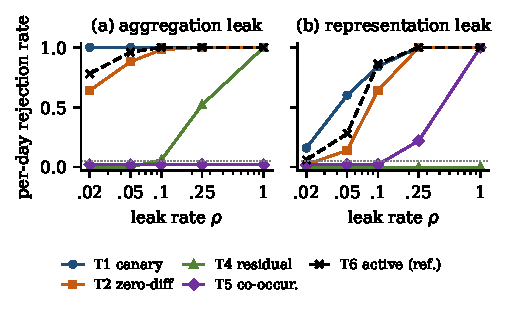
\includegraphics[width=\columnwidth]{power.pdf}
\caption{Per-day rejection rate ($\alpha=0.05$) against the fraction $\rho$ of opted-out edges leaked, averaged over 5 seeds $\times$ 10 days. Rows: leak pattern. Columns: leakage channel. Dotted line: nominal level. Dashed black: the T7 reference with 20 canary accounts and 80 canary edges per day. T4 targets aggregates only; T5 and T6 target representation leakage only.}
\label{fig:power}
\end{figure}

\begin{table}[t]
\centering\footnotesize
\setlength{\tabcolsep}{3pt}
\begin{tabular}{@{}lccccc@{}}
\toprule
 & \multicolumn{5}{c}{leak rate $\rho$} \\
\cmidrule(l){2-6}
Leak / channel / tests & .02 & .05 & .10 & .25 & 1.0 \\
\midrule
\multicolumn{6}{@{}l}{\emph{Per-edge leaks}} \\
Aggregation, passive & 5/5 (1) & 5/5 (1) & 5/5 (1) & 5/5 (1) & 5/5 (1) \\
Aggregation, T7      & 5/5 (1) & 5/5 (1) & 5/5 (1) & 5/5 (1) & 5/5 (1) \\
Representation, passive & 0/5 & 3/5 (3) & 5/5 (2) & 5/5 (1) & 5/5 (1) \\
Representation, T7      & 0/5 & 4/5 (4.5) & 5/5 (2) & 5/5 (2) & 5/5 (2) \\
\multicolumn{6}{@{}l}{\emph{Per-customer leaks}} \\
Aggregation, passive & 5/5 (1) & 5/5 (1) & 5/5 (1) & 5/5 (1) & 5/5 (1) \\
Aggregation, T7      & 2/5 (1) & 5/5 (1) & 5/5 (1) & 5/5 (1) & 5/5 (1) \\
Representation, passive & 5/5 (7) & 5/5 (2) & 5/5 (1) & 5/5 (1) & 5/5 (1) \\
Representation, T7      & 2/5 (5.5) & 5/5 (5) & 5/5 (2) & 5/5 (2) & 5/5 (2) \\
\midrule
Clean, passive and T7 & \multicolumn{5}{c}{0/30 false alarms each} \\
\bottomrule
\end{tabular}
\caption{Audits in which the e-process reached $20$ within 10 days (median detection day in parentheses). ``Passive'' averages the e-processes of T1, T2, T4, T5 and T6; T7 uses 20 canary accounts and 80 canary edges per day.}
\label{tab:detect}
\end{table}

\paragraph{Power.}
Figure~\ref{fig:power} and Table~\ref{tab:detect} summarize the results.

\emph{Per-edge leaks, aggregation.} T1 alone rejects on every day even at
$\rho=0.02$, which leaks roughly 0.2\% of all edges. An opted-out customer with
any leaked edge has a non-default feature, and the exact check catches it.
T2's exact aggregate check follows closely. T4 needs $\rho\ge 0.25$, because
summarizing $\Eout$ by degree throws away the identity of the leaked edges.

\emph{Per-edge leaks, representation} are harder. The combined passive
e-process detects them by day 2 (median) at $\rho=0.1$, and in 3 of 5 audits at
$\rho=0.05$. T1 is again the most powerful single test: the factorization
assigns a nonzero embedding to canary items whose training column is no
longer empty. T5 detects only $\rho\ge 0.25$, and T6 only $\rho=1$. This is the
$\rho^2$ effect predicted in Section~\ref{sec:tests}: a link between two items
needs two leaked edges of the same customer.

\emph{Per-customer leaks} change the picture for the co-interaction tests.
When whole customers leak, their edges leak together, so T5 rejects on 88\%
of days and T6 on 50\% at $\rho=0.25$, against 22\% and 4\% for per-edge leaks.
T6's effect size $\lambda$ now tracks the leak rate: its median is 0.29 at
$\rho=0.25$ and 0.98 at $\rho=1$. It is biased upward by about 0.09, its median on
clean days, so it is informative only well above that level. The combined
passive e-process detects every per-customer leak, including $\rho=0.02$ in the
representation, where the median detection day is 7. The learned T6 scorer
behaves like the cosine score throughout. Its per-day rejection rates differ
by at most 0.06.

\emph{Passive tests against the T7 reference.} T7 is exactly valid, with zero
false alarms, and detects every leak with $\rho\ge 0.1$. The passive T1 matches
or beats it in every setting except one: per-edge representation leakage at
$\rho=0.1$, where T7 rejects on 86\% of days and T1 on 84\%. For per-edge leaks,
the reason is budget: natural opt-outs supply about 30 times more ``canary
edges'' per day than our 80 synthetic ones, at no cost. For per-customer
leaks, the gap is starker, because T7 becomes a lottery. With 20 canary
accounts and $\rho=0.02$, the chance that any canary account leaks is
$1-0.98^{20}\approx 33\%$, and T7 detects only 2 of 5 audits. The roughly 300
natural opted-out customers contain about 6 leaking customers on any day.
Two lessons follow. First, a passive audit built on natural canaries can be
as powerful as a modest active campaign, without write access. Under
per-customer leakage, an active campaign should spend its budget on many
accounts rather than many edges per account. Second, T7's value lies in its
guaranteed validity, not its power. It checks the passive tests on the real
pipeline, where their assumptions cannot be verified directly.

%---------------------------------------------------------------------
\subsection{Real data: RetailRocket}\label{sec:real}
\paragraph{Data.}
We use the public RetailRocket e-commerce event log~\citep{retailrocket}. It
covers 4.5 months and contains 2.66M views, 69k add-to-carts and 22k
transactions by 1.4M visitors on 235k items. We drop visitors with fewer than
2 or more than 200 events. Single events carry no co-interaction, and the
heaviest visitors are mostly crawlers. That leaves 405{,}832 customers and
162{,}225 items. The log has no merchant field, so our real-data audits cover
customers and items only.

\paragraph{Semi-synthetic design.}
The interaction graph is real. Opt-outs and leaks are simulated, because real
consent labels are not public. The snapshot for day $t$ contains the typed edges
of the window $[t-6,t]$, one per (customer, item) pair with the strongest event
type, about 60k edges per day. Intrinsic item embeddings come from an SVD of
days 0--29, which no audit window includes. Opt-out status, pipelines and leak
patterns are as in the simulator. Each audit covers 10--14 days, starting on
day 37.

\begin{table}[t]
\centering\footnotesize
\setlength{\tabcolsep}{3pt}
\begin{tabular}{@{}lcccccc@{}}
\toprule
 & Clean & \multicolumn{2}{c}{Aggregation} & \multicolumn{3}{c}{Representation} \\
\cmidrule(lr){3-4}\cmidrule(l){5-7}
Test & FPR & .1 & 1.0 & .1 & .1 cust. & 1.0 \\
\midrule
T1 & 0 & 100 & 100 & 100 & -- & 100 \\
T2 & 0 & 100 & 100 & 0 & -- & 100 \\
T4$^*$ & 17 & 100 & 100 & 0 & -- & 15 \\
T5 basic$^*$ & 29 & -- & -- & 60 & 85 & 100 \\
T5 refined & 0 & -- & -- & 0 & 5 & 100 \\
T6 basic$^*$ & 13 & -- & -- & 10 & 15 & 90 \\
T6 refined & 0 & -- & -- & 0 & 5 & 100 \\
\bottomrule
\end{tabular}
\caption{RetailRocket, per-day rejection rate (\%). Clean: false-alarm rate on compliant pipelines (42 days for T1, T2 and T4; 98 for basic T5 and T6; 56 for refined). Leak columns give the leak rate $\rho$, with per-edge leakage unless marked ``cust.''; 2 opt-out draws $\times$ 10 days. $^*$Not calibrated on real data, so its power is not meaningful.}
\label{tab:real}
\end{table}

\paragraph{Structural tests hold.}
T1 and T2 raise no false alarm on 42 compliant days (Table~\ref{tab:real}). The
real long tail supplies about 1{,}900 natural canary items per day, against 34
in the simulator. As a result, T1 rejects on every day for every leak in our
grid, including per-edge representation leakage at $\rho=0.1$, where every
other calibrated test is blind. Its e-process raises an alarm on day 1 for
aggregation leaks and on day 2 for representation leaks. With 2{,}000
permutations, a single day's p-value cannot fall below $1/2001$, so one day of
evidence falls just short of the threshold. More permutations would bring the
alarm to day 1.

\paragraph{Behavioral tests need the refinements.}
The basic T4, T5 and T6 rely on exchangeable behavior, and they alarm on 17\%,
29\% and 13\% of compliant days (P5). The refined T5 and T6 raise no false alarm
on 56 compliant days. They keep full power at $\rho=1$, but detect little at
$\rho=0.1$ (0--5\% of days). On synthetic data, the refined T5 alarms on 7.5\% of
200 compliant days, slightly above the nominal 5\%, and the refined T6 on 5\%.
There, the refined T6 is more powerful than the basic one under per-customer
leakage (70\% against 48\% of days at $\rho=0.25$), and the refined T5 is less
powerful (56\% against 74\%). T4 remains miscalibrated on real data. Items that
share customers are dependent, and a cluster-robust version is future work. We
therefore exclude T4 from real-data alarms.

\paragraph{Takeaway.}
Real behavior separates the tests into two groups. Tests built on structural
facts, an empty or unchanged receptive field (T1, T2), carry over from the
simulator unchanged and stay powerful. Tests built on behavioral
exchangeability (T4, T5, T6) are sound in the simulator but need cluster-aware
units and time-bracketed references on real data. A null study on real data
is therefore not optional. It is what revealed P5.

%---------------------------------------------------------------------
\subsection{Feature families as test targets}\label{sec:families}
The pipelines above mix several feature types into one vector. Real feature
stores keep them apart, and a leak usually affects one job. We therefore
implement one representative of each family of Table~\ref{tab:families} and
test each one separately.

\paragraph{Targets.}
A1 holds an item's typed counts and number of unique customers; A2, its
conversion share (purchase-like edges over all edges) and mean interaction
type; A3, a count decayed with a half-life of two days (real data only, since
the simulator keeps no dates). R1 is a rank-16 randomized SVD of the
type-weighted customer--item matrix, reseeded daily. R2 is a rank-16 SVD of the
positive PMI matrix of item co-occurrence, the factorization that skip-gram
item embeddings approximate~\citep{levy2014neural}. R3 is a LightGCN-style
propagation of R1: half the item's own factor, half the mean factor of the
items that share a customer with it. R4 averages the attributes $z$ (gender,
birth year, a two-dimensional residence) of an item's customers. In the
simulator, $z$ is correlated with each customer's preferences; RetailRocket
publishes no attributes, so we draw them at random. Customer features average
the item features over the customer's edges. A leaking job computes its
feature from $\Ein$ plus the leaked opted-out edges, together with the
attributes of the customers behind them in R4. We use per-customer leakage,
the more common pattern, at $\rho=0.1$ and $\rho=1$.

\paragraph{Tests.}
T1 compares canaries with cold items. In all seven jobs, an item with no
opted-in edge receives a deterministic default (a zero vector), so T1 is an
exact check: any canary that differs from the default is a violation. T2 is
exact for the 1-hop deterministic jobs (A1, A2, R4) and uses the aligned
regression otherwise, with 2-hop invariance. T5 and T6 run on the
representations, with the refinements of Pitfall~5.

\begin{table}[t]
\centering\footnotesize
\setlength{\tabcolsep}{2.6pt}
\begin{tabular}{@{}llcccccc@{}}
\toprule
 & & \multicolumn{3}{c}{Simulator} & \multicolumn{3}{c}{RetailRocket} \\
\cmidrule(lr){3-5}\cmidrule(l){6-8}
 & Test & clean & $0.1$ & $1$ & clean & $0.1$ & $1$ \\
\midrule
A1 & T1 & 0 & 100 & 100 & 0 & 100 & 100 \\
 & T2 & 0 & 100 & 100 & 0 & 100 & 100 \\
\addlinespace[1pt]
A2 & T1 & 0 & 100 & 100 & 0 & 100 & 100 \\
 & T2 & 0 & 97 & 100 & 0 & 100 & 100 \\
\addlinespace[1pt]
A3 & T1 & -- & -- & -- & 0 & 100 & 100 \\
 & T2 & -- & -- & -- & 0 & 21 & 100 \\
\addlinespace[1pt]
R1 & T1 & 0 & 100 & 100 & 0 & 100 & 100 \\
 & T2 & 2 & 7 & 100 & 10 & 36 & 100 \\
 & T5 & 2 & 10 & 100 & 5 & 79 & 100 \\
 & T6 & 3 & 3 & 97 & 0 & 14 & 100 \\
\addlinespace[1pt]
R2 & T1 & 0 & 100 & 100 & 0 & 100 & 100 \\
 & T2 (2-hop) & 5 & 7 & 93 & 48 & 79 & 100 \\
 & T2 (+3-hop churn) & 5 & 7 & 93 & 10 & 7 & 100 \\
 & T5 & 1 & 33 & 100 & 5 & 57 & 100 \\
 & T6 & 0 & 7 & 90 & 0 & 0 & 100 \\
\addlinespace[1pt]
R3 & T1 & 0 & 100 & 100 & 0 & 100 & 100 \\
 & T2 & 2 & 23 & 100 & 10 & 43 & 100 \\
 & T5 & 0 & 10 & 100 & 5 & 86 & 100 \\
 & T6 & 6 & 13 & 63 & 0 & 7 & 100 \\
\addlinespace[1pt]
R4 & T1 & 0 & 100 & 100 & 0 & 100 & 100 \\
 & T2 & 0 & 100 & 100 & 0 & 100 & 100 \\
 & T5 & 6 & 23 & 97 & 0 & 29 & 100 \\
 & T6 & 7 & 7 & 27 & 10 & 21 & 100 \\
\bottomrule
\end{tabular}
\caption{Per-day rejection rate (\%, $\alpha=0.05$) for each feature family of Table~\ref{tab:families} tested separately. ``Clean'' is the false-alarm rate on compliant jobs (100 simulated and 21 real days); $0.1$ and $1$ are per-customer leak rates $\rho$ (30 simulated and 14 real days each).}
\label{tab:famres}
\end{table}

\paragraph{Results.}
Table~\ref{tab:famres} shows four patterns.
\begin{itemize}
  \item \emph{Local features are verified exactly.} For counts, rates and
        attribute aggregation (A1, A2, R4), T1 and T2 never raise a false
        alarm and catch every leaking day, even at $\rho=0.1$. R4 shows that
        an attribute leak, where items absorb who opted-out customers are, is
        as easy to catch as a count leak. The decayed count (A3) changes every
        day by design, so T2 loses exactness and its power at $\rho=0.1$ drops
        to 21\%; T1 remains exact.
  \item \emph{Natural canaries carry the representations.} T1 catches every
        leaking day for R1--R3 on both data sources, because a leaked
        customer's niche items stop sitting at the cold default. This relies
        on a deterministic default for never-seen items; a pipeline that
        initializes them at random needs the permutation version of T1
        (Section~\ref{sec:tests}).
  \item \emph{Global representations are hard for the other tests at low leak
        rates.} At $\rho=0.1$, T2, T5 and T6 detect 3--33\% of simulated days
        for R1--R3, and 7--86\% of real days, with T5 the strongest. At
        $\rho=1$ every test detects every or almost every day, except T6 on R3
        (63\%) and R4 (27\%) in the simulator.
  \item \emph{The receptive field must match the feature (Pitfall~1).} R2's
        PMI weights divide by the co-occurrence totals of neighboring items,
        so its receptive field is three hops, not two. With 2-hop invariance,
        T2 alarms on 48\% of compliant real days. Adjusting the T2 regression
        for opted-in churn at the third hop restores calibration (10\%, i.e.,
        2 of 21 days) but costs most of its power at $\rho=0.1$. The same
        adjustment over-corrects R1 and R3, so we apply it only where the
        receptive field calls for it.
\end{itemize}
The remaining false-alarm rates of 6--10\% (R4 under T5 and T6, R1 and R3
under T2 on real data) correspond to at most 2 of 21 real days or 7 of 100
simulated days; they are compatible with the nominal 5\% at these sample
sizes, but larger null studies would be needed to confirm calibration per
family.


%=====================================================================
\section{Related Work}\label{sec:related}
%=====================================================================
To our knowledge, no prior work audits opt-out compliance of a feature
pipeline from its inputs and outputs alone. Several lines of work come close,
and each differs in a way that matters for our setting.

\paragraph{Auditing consent compliance.}
\citet{liu2024optedout} audit whether advertisers honor opt-outs signaled
through consent management platforms. They infer data use from advertisers'
bidding behavior and find that several ad platforms ignore consent. Their
auditor, like ours, sees only external behavior. The object is different,
though. They measure whether third parties collect and share data, not how a
first party's derived features depend on opted-out records. From the legal
side, \citet{biega2021reviving} analyze purpose limitation in data-driven
systems and note that black-box methods for auditing such compliance had not
been developed.

\paragraph{Data-use auditing and membership inference.}
Membership inference asks whether a record was in a model's training
set~\citep{shokri2017membership,carlini2022first}. For recommender systems,
\citet{zhang2021membership} infer whether a user's history was used from the
recommendations alone. \citet{huang2024general} turn membership inference into
\emph{proactive} data-use auditing. A data owner publishes one of two marked
versions of each record and applies a sequential test with a controlled
false-detection rate. These works audit a single trained model with query
access, usually for data the auditor itself marked. Our T6 and T7 borrow these
ideas. The passive tests (T1--T6) instead exploit natural experiments in
continuously recomputed graph features, where removal must also propagate to
neighbors and the main obstacle is confounding by correlated behavior
(Section~\ref{sec:challenges}).

\paragraph{Verifying unlearning.}
Athena~\citep{sommer2022athena} verifies deletion requests by having some users
plant backdoors in their data and testing whether the backdoor survives.
\citet{eisenhofer2025verifiable} require the server to produce cryptographic
proofs of training and unlearning. \citet{thudi2022necessity} show that the
model parameters alone cannot certify that a point was unlearned, which echoes
our Proposition~\ref{prop:imposs}. Unlearning
methods~\citep{ginart2019making,bourtoule2021machine}, including graph and
recommendation variants~\citep{chen2022graph,chen2022recommendation}, make
removal efficient, but they are mechanisms, not audits. Our setting differs in three ways.
Opt-outs are continuous rather than one-off requests, the auditor has no
query access to a model, and the influence of removed data spreads through
the graph.

\paragraph{Privacy auditing.}
Empirical DP auditing inserts canaries and measures distinguishability to
lower-bound privacy loss~\citep{jagielski2020auditing,nasr2021adversary,steinke2023one}.
Our tests can be read as auditing a degenerate mechanism that should have
$\varepsilon=0$ with respect to $\Eout$. The auditor usually cannot choose the
inputs, which is why we rely on natural experiments, and the reference
distribution must be built from correlated behavioral data rather than from a
known mechanism.

\paragraph{Enforcement inside the system.}
Industry also enforces consent and purpose limitation from the inside. Meta's
Policy Zones, for example, attach purpose annotations to data and track
information flow at runtime across its warehouse and serving
stacks~\citep{meta2024pai}. Such white-box controls and our black-box audit
complement each other. Information-flow control prevents violations where it
is deployed. Output-based auditing checks the result independently, including
components that the enforcement layer does not cover.

\paragraph{Graph privacy attacks.}
Link stealing and GNN membership
inference~\citep{he2021stealing,olatunji2021membership} show that node outputs
reveal edges. T5 and T6 turn these attacks into audit statistics, with
references that separate memorization from homophily.

%=====================================================================
\section{Limitations}\label{sec:limits}
%=====================================================================
Our real-data study is semi-synthetic: the interactions are real, but opt-outs
and leaks are simulated, and RetailRocket has no merchant layer. Real opt-out
decisions may correlate with behavior. Privacy-conscious customers may browse
differently, which would add confounding beyond P5. Before deployment, every
test should first be run on days or slices where compliance is known, such
as a pipeline replica fed only $\Ein$. That is how we found P5. T4 is not
calibrated on real data, and the refined T5 is slightly anti-conservative in
the simulator (7.5\%). Assumption~\ref{ass:local} and the exchangeability behind
the placebo references are modeling choices that seasonality or product
launches can break. T7 depends on neither, which is why we recommend periodic
canary campaigns wherever write access exists. Daily e-values are not strictly
independent. Finally, Proposition~\ref{prop:imposs} bounds what any of this can
achieve against a pipeline that leaks deliberately and sparsely. Code audits,
data lineage and attested execution remain necessary complements.

%=====================================================================
\section{Conclusion}
%=====================================================================
Opt-out compliance in black-box graph feature pipelines cannot be proven
from outputs, but it can be falsified efficiently. The most effective
evidence comes from nodes whose correct output is known in advance: natural
canaries and invariant neighborhoods. These carry over from synthetic to
real data unchanged. Validity, however, depends on details: typed edges, an
agreed opt-out policy, symmetric references, and units that respect how real
customers browse. Our real-data null study exposed the last of these, which
the simulator could not. Every audit should therefore begin with a null study
on real data, and its result should be reported as a calibrated detection
bound.

\footnotesize
\begin{thebibliography}{99}
\setlength{\itemsep}{1pt}

\bibitem[Angrist and Pischke(2009)]{angrist2009mostly}
Angrist, J.~D., and Pischke, J.-S. 2009.
\newblock \emph{Mostly Harmless Econometrics}. Princeton University Press.

\bibitem[Barkan and Koenigstein(2016)]{barkan2016item2vec}
Barkan, O.; and Koenigstein, N. 2016.
\newblock Item2vec: Neural item embedding for collaborative filtering.
\newblock In \emph{IEEE International Workshop on Machine Learning for Signal Processing (MLSP)}.

\bibitem[Biega and Finck(2021)]{biega2021reviving}
Biega, A.~J., and Finck, M. 2021.
\newblock Reviving purpose limitation and data minimisation in data-driven systems.
\newblock \emph{Technology and Regulation} 2021:44--61.

\bibitem[Borisyuk et~al.(2024)]{borisyuk2024lignn}
Borisyuk, F.; He, S.; Ouyang, Y.; Ramezani, M.; Du, P.; et~al. 2024.
\newblock LiGNN: Graph neural networks at LinkedIn.
\newblock In \emph{KDD}.

\bibitem[Bourtoule et~al.(2021)]{bourtoule2021machine}
Bourtoule, L.; Chandrasekaran, V.; Choquette-Choo, C.~A.; et~al. 2021.
\newblock Machine unlearning.
\newblock In \emph{IEEE Symposium on Security and Privacy}.

\bibitem[Carlini et~al.(2019)]{carlini2019secret}
Carlini, N.; Liu, C.; Erlingsson, {\'U}.; Kos, J.; and Song, D. 2019.
\newblock The secret sharer: Evaluating and testing unintended memorization in neural networks.
\newblock In \emph{USENIX Security Symposium}.

\bibitem[Carlini et~al.(2022)]{carlini2022first}
Carlini, N.; Chien, S.; Nasr, M.; Song, S.; Terzis, A.; and Tram{\`e}r, F. 2022.
\newblock Membership inference attacks from first principles.
\newblock In \emph{IEEE Symposium on Security and Privacy}.

\bibitem[Chen et~al.(2022a)]{chen2022graph}
Chen, M.; Zhang, Z.; Wang, T.; Backes, M.; Humbert, M.; and Zhang, Y. 2022a.
\newblock Graph unlearning.
\newblock In \emph{ACM CCS}.

\bibitem[Chen et~al.(2022b)]{chen2022recommendation}
Chen, C.; Sun, F.; Zhang, M.; and Ding, B. 2022b.
\newblock Recommendation unlearning.
\newblock In \emph{The Web Conference (WWW)}.

\bibitem[Cheng et~al.(2016)]{cheng2016wide}
Cheng, H.-T.; Koc, L.; Harmsen, J.; et~al. 2016.
\newblock Wide \& deep learning for recommender systems.
\newblock In \emph{Workshop on Deep Learning for Recommender Systems (DLRS)}.

\bibitem[Chernozhukov et~al.(2018)]{chernozhukov2018double}
Chernozhukov, V.; Chetverikov, D.; Demirer, M.; Duflo, E.; Hansen, C.; Newey, W.; and Robins, J. 2018.
\newblock Double/debiased machine learning for treatment and structural parameters.
\newblock \emph{The Econometrics Journal} 21(1).

\bibitem[Covington, Adams, and Sargin(2016)]{covington2016deep}
Covington, P.; Adams, J.; and Sargin, E. 2016.
\newblock Deep neural networks for {YouTube} recommendations.
\newblock In \emph{ACM RecSys}.

\bibitem[Eisenhofer et~al.(2025)]{eisenhofer2025verifiable}
Eisenhofer, T.; Riepel, D.; Chandrasekaran, V.; Ghosh, E.; Ohrimenko, O.; and Papernot, N. 2025.
\newblock Verifiable and provably secure machine unlearning.
\newblock In \emph{IEEE SaTML}.

\bibitem[El-Kishky et~al.(2022)]{elkishky2022twhin}
El-Kishky, A.; Markovich, T.; Park, S.; Verma, C.; Kim, B.; Eskander, R.; Malkov, Y.; Portman, F.; Samaniego, S.; Xiao, Y.; and Haghighi, A. 2022.
\newblock TwHIN: Embedding the Twitter heterogeneous information network for personalized recommendation.
\newblock In \emph{KDD}.

\bibitem[Fey and Lenssen(2019)]{fey2019pyg}
Fey, M., and Lenssen, J.~E. 2019.
\newblock Fast graph representation learning with PyTorch Geometric.
\newblock In \emph{ICLR Workshop on Representation Learning on Graphs and Manifolds}.

\bibitem[Frasca et~al.(2020)]{frasca2020sign}
Frasca, F.; Rossi, E.; Eynard, D.; Chamberlain, B.; Bronstein, M.; and Monti, F. 2020.
\newblock SIGN: Scalable inception graph neural networks.
\newblock \emph{arXiv:2004.11198}.

\bibitem[Ginart et~al.(2019)]{ginart2019making}
Ginart, A.; Guan, M.; Valiant, G.; and Zou, J. 2019.
\newblock Making AI forget you: Data deletion in machine learning.
\newblock In \emph{NeurIPS}.

\bibitem[Grbovic and Cheng(2018)]{grbovic2018real}
Grbovic, M., and Cheng, H. 2018.
\newblock Real-time personalization using embeddings for search ranking at Airbnb.
\newblock In \emph{KDD}.

\bibitem[Grover and Leskovec(2016)]{grover2016node2vec}
Grover, A.; and Leskovec, J. 2016.
\newblock node2vec: Scalable feature learning for networks.
\newblock In \emph{ACM KDD}.

\bibitem[Halko, Martinsson, and Tropp(2011)]{halko2011finding}
Halko, N.; Martinsson, P.-G.; and Tropp, J.~A. 2011.
\newblock Finding structure with randomness: Probabilistic algorithms for constructing approximate matrix decompositions.
\newblock \emph{SIAM Review} 53(2).

\bibitem[Hamilton, Ying, and Leskovec(2017)]{hamilton2017graphsage}
Hamilton, W.; Ying, Z.; and Leskovec, J. 2017.
\newblock Inductive representation learning on large graphs.
\newblock In \emph{NeurIPS}.

\bibitem[He et~al.(2020)]{he2020lightgcn}
He, X.; Deng, K.; Wang, X.; Li, Y.; Zhang, Y.; and Wang, M. 2020.
\newblock LightGCN: Simplifying and powering graph convolution network for recommendation.
\newblock In \emph{SIGIR}.

\bibitem[He et~al.(2021)]{he2021stealing}
He, X.; Jia, J.; Backes, M.; Gong, N.~Z.; and Zhang, Y. 2021.
\newblock Stealing links from graph neural networks.
\newblock In \emph{USENIX Security Symposium}.

\bibitem[Hermann and Del~Balso(2017)]{hermann2017michelangelo}
Hermann, J., and Del~Balso, M. 2017.
\newblock Meet Michelangelo: Uber's machine learning platform.
\newblock Uber Engineering Blog. \url{https://www.uber.com/blog/michelangelo-machine-learning-platform/}.

\bibitem[Huang, Gong, and Reiter(2024)]{huang2024general}
Huang, Z.; Gong, N.~Z.; and Reiter, M.~K. 2024.
\newblock A general framework for data-use auditing of ML models.
\newblock In \emph{ACM CCS}.

\bibitem[Jagielski, Ullman, and Oprea(2020)]{jagielski2020auditing}
Jagielski, M.; Ullman, J.; and Oprea, A. 2020.
\newblock Auditing differentially private machine learning: How private is private SGD?
\newblock In \emph{NeurIPS}.

\bibitem[Koch(2018)]{koch2018doordash}
Koch, M. 2018.
\newblock Personalized store feed with vector embeddings.
\newblock DoorDash Engineering Blog.

\bibitem[Koren, Bell, and Volinsky(2009)]{koren2009matrix}
Koren, Y.; Bell, R.; and Volinsky, C. 2009.
\newblock Matrix factorization techniques for recommender systems.
\newblock \emph{Computer} 42(8): 30--37.

\bibitem[Levy and Goldberg(2014)]{levy2014neural}
Levy, O.; and Goldberg, Y. 2014.
\newblock Neural word embedding as implicit matrix factorization.
\newblock In \emph{NeurIPS}.

\bibitem[Liu et~al.(2022)]{liu2022a2gcn}
Liu, F.; Cheng, Z.; Zhu, L.; Liu, C.; and Nie, L. 2022.
\newblock An attribute-aware attentive {GCN} model for attribute missing in recommendation.
\newblock \emph{IEEE Transactions on Knowledge and Data Engineering} 34(9): 4077--4088.

\bibitem[Liu, Iqbal, and Saxena(2024)]{liu2024optedout}
Liu, Z.; Iqbal, U.; and Saxena, N. 2024.
\newblock Opted out, yet tracked: Are regulations enough to protect your privacy?
\newblock \emph{Proceedings on Privacy Enhancing Technologies} 2024(1):280--299.

\bibitem[Meta(2024)]{meta2024pai}
Meta. 2024.
\newblock Engineering at Meta blog post on Privacy Aware Infrastructure and purpose limitation with Policy Zones.
\newblock \url{https://engineering.fb.com/2024/08/27/security/privacy-aware-infrastructure-purpose-limitation-meta/}.

\bibitem[Nasr et~al.(2021)]{nasr2021adversary}
Nasr, M.; Song, S.; Thakurta, A.; Papernot, N.; and Carlini, N. 2021.
\newblock Adversary instantiation: Lower bounds for differentially private machine learning.
\newblock In \emph{IEEE Symposium on Security and Privacy}.

\bibitem[Olatunji, Nejdl, and Khosla(2021)]{olatunji2021membership}
Olatunji, I.~E.; Nejdl, W.; and Khosla, M. 2021.
\newblock Membership inference attack on graph neural networks.
\newblock In \emph{IEEE TPS-ISA}.

\bibitem[Ramdas et~al.(2023)]{ramdas2023game}
Ramdas, A.; Gr{\"u}nwald, P.; Vovk, V.; and Shafer, G. 2023.
\newblock Game-theoretic statistics and safe anytime-valid inference.
\newblock \emph{Statistical Science} 38(4).

\bibitem[RetailRocket(2016)]{retailrocket}
RetailRocket. 2016.
\newblock Retailrocket recommender system dataset.
\newblock Kaggle. \url{https://www.kaggle.com/retailrocket/ecommerce-dataset}.

\bibitem[Sarda et~al.(2019)]{sarda2019ubereats}
Sarda, A.; Jain, A.; Liu, I.; et~al. 2019.
\newblock Food discovery with Uber Eats: Using graph learning to power recommendations.
\newblock Uber Engineering Blog. \url{https://www.uber.com/blog/uber-eats-graph-learning/}.

\bibitem[Sch{\"o}nemann(1966)]{schonemann1966procrustes}
Sch{\"o}nemann, P.~H. 1966.
\newblock A generalized solution of the orthogonal Procrustes problem.
\newblock \emph{Psychometrika} 31(1).

\bibitem[Shafer et~al.(2011)]{shafer2011test}
Shafer, G.; Shen, A.; Vereshchagin, N.; and Vovk, V. 2011.
\newblock Test martingales, Bayes factors and p-values.
\newblock \emph{Statistical Science} 26(1).

\bibitem[Shah and Peters(2020)]{shah2020hardness}
Shah, R.~D., and Peters, J. 2020.
\newblock The hardness of conditional independence testing and the generalised covariance measure.
\newblock \emph{The Annals of Statistics} 48(3).

\bibitem[Shokri et~al.(2017)]{shokri2017membership}
Shokri, R.; Stronati, M.; Song, C.; and Shmatikov, V. 2017.
\newblock Membership inference attacks against machine learning models.
\newblock In \emph{IEEE Symposium on Security and Privacy}.

\bibitem[Sommer et~al.(2022)]{sommer2022athena}
Sommer, D.~M.; Song, L.; Wagh, S.; and Mittal, P. 2022.
\newblock Athena: Probabilistic verification of machine unlearning.
\newblock \emph{Proceedings on Privacy Enhancing Technologies} 2022(3):268--290.

\bibitem[Steinke, Nasr, and Jagielski(2023)]{steinke2023one}
Steinke, T.; Nasr, M.; and Jagielski, M. 2023.
\newblock Privacy auditing with one (1) training run.
\newblock In \emph{NeurIPS}.

\bibitem[Tianchi(2018)]{taobao2018}
Alibaba Tianchi. 2018.
\newblock User behavior data from Taobao for recommendation.
\newblock \url{https://tianchi.aliyun.com/dataset/649}.

\bibitem[Thudi et~al.(2022)]{thudi2022necessity}
Thudi, A.; Jia, H.; Shumailov, I.; and Papernot, N. 2022.
\newblock On the necessity of auditable algorithmic definitions for machine unlearning.
\newblock In \emph{USENIX Security Symposium}.

\bibitem[Tianchi(2015)]{tmall2015}
Alibaba Tianchi. 2015.
\newblock Repeat buyers prediction after sales promotion (IJCAI-15 competition dataset).
\newblock \url{https://tianchi.aliyun.com/}.

\bibitem[Vovk and Wang(2021)]{vovk2021evalues}
Vovk, V., and Wang, R. 2021.
\newblock E-values: Calibration, combination and applications.
\newblock \emph{The Annals of Statistics} 49(3).

\bibitem[Wang et~al.(2018)]{wang2018billion}
Wang, J.; Huang, P.; Zhao, H.; Zhang, Z.; Zhao, B.; and Lee, D.~L. 2018.
\newblock Billion-scale commodity embedding for e-commerce recommendation in Alibaba.
\newblock In \emph{KDD}.

\bibitem[Yi et~al.(2019)]{yi2019sampling}
Yi, X.; Yang, J.; Hong, L.; Cheng, D.~Z.; Heldt, L.; Kumthekar, A.; Zhao, Z.; Wei, L.; and Chi, E. 2019.
\newblock Sampling-bias-corrected neural modeling for large corpus item recommendations.
\newblock In \emph{ACM RecSys}.

\bibitem[Ying et~al.(2018)]{ying2018graph}
Ying, R.; He, R.; Chen, K.; Eksombatchai, P.; Hamilton, W.~L.; and Leskovec, J. 2018.
\newblock Graph convolutional neural networks for web-scale recommender systems.
\newblock In \emph{KDD}.

\bibitem[Zhang et~al.(2021)]{zhang2021membership}
Zhang, M.; Ren, Z.; Wang, Z.; Ren, P.; Chen, Z.; Hu, P.; and Zhang, Y. 2021.
\newblock Membership inference attacks against recommender systems.
\newblock In \emph{ACM CCS}.

\bibitem[Zhu et~al.(2019)]{zhu2019aligraph}
Zhu, R.; Zhao, K.; Yang, H.; Lin, W.; Zhou, C.; Ai, B.; Li, Y.; and Zhou, J. 2019.
\newblock AliGraph: A comprehensive graph neural network platform.
\newblock \emph{PVLDB} 12(12).

\end{thebibliography}

\end{document}
